\documentclass[12pt,a4paper,oneside,openany]{memoir} 
% Skabelon af DTU's LaTeX support gruppe, v20090423

\usepackage[utf8x]{inputenc}
%\usepackage[danish]{babel} % danske overskrifter
\usepackage[T1]{fontenc}   % fonte (output)
\usepackage{lmodern}       % vektor fonte
\usepackage{fancybox, graphicx}      % indsættelse af billeder
\usepackage{palatino}      % lækker font
\usepackage{pdfpages}      % pdf som forside evt
\usepackage{todonotes}
\usepackage{microtype}
\usepackage{amsmath,amstext,amsthm,import}
\usepackage{ulem}
\usepackage{float}
\usepackage{xparse}
\usepackage{array}
\usepackage{usecases}
\usepackage{pdfpages}
\usepackage{slashbox}
% \linespread{1.3}           % kræver lidt mere line spacing

\newcommand{\code}[1]{\texttt{#1}}
\newcommand{\HRule}{\rule{\linewidth}{0.5mm}}

%\addto\captionsdanish{
%  \renewcommand{\contentsname}%
%    {Indholdsfortegnelse}     %
%} % Så bruger vi bare 'Indholdsfortegnelse' i stedet for 'Indhold'


\usepackage{underscore}
\usepackage{pdflscape}
\usepackage{todonotes}

\usepackage[plainpages=false,pdfpagelabels,pageanchor=false]{hyperref} % aktive links
\def\sectionautorefname{afsnit}

\usepackage{memhfixc}  % rettelser til hyperref
\hypersetup{%
    pdfborder = {0 0 0}
}
\usepackage{tipa}
\pretolerance=2500     % højt tal, mindre orddeling og mere space mellem ord.
% 3000 er okey, 1000 er for lidt, 5000 i overkanten, 8000 er for meget..

\usepackage[font=small,labelfont=bf,labelsep=endash]{caption}
 
\pagestyle{headings}


\makechapterstyle{mortenovi}{%
\setlength{\beforechapskip}{0cm}%længde fra top af side til kapitel-overskrifter
\setlength{\afterchapskip}{1cm}%længde fra kapiteltekst til body-tekst
\setlength{\midchapskip}{2cm}%længe mellem kapitelnummer og kapiteltekst
\renewcommand\chapnamefont{\normalfont\Large\scshape\raggedleft}
\renewcommand\chaptitlefont{\normalfont\Huge\bfseries\sffamily}
\renewcommand\chapternamenum{}%default "kapitel"
\renewcommand\printchapternum{%
    \makebox[0pt][l]{%
    \hspace{0.4em}
    \resizebox{!}{4ex}{\chapnamefont\bfseries\sffamily\thechapter}}
    }%"kapitel. x"-linjen og dens boxe og bredder - prøv at sætte xyz ind først på de tre linjer respektivt.
\renewcommand\afterchapternum{\par\hspace{1.5cm}\hrule\vspace{0.5cm}}
\renewcommand\afterchaptertitle{\vskip\onelineskip \hrule\vskip\afterchapskip
}}
\chapterstyle{mortenovi}

\maxtocdepth{subsection} %Only parts, chapters and sections in the table of contents
\settocdepth{subsection}

% \includeonly{forord,testing} % Kompiler kun de kapitler du arbejder med.

\usepackage{listings}
\usepackage{color}

\renewcommand*\lstlistingname{Kode}

\definecolor{dkgreen}{rgb}{0,0.6,0}
\definecolor{gray}{rgb}{0.5,0.5,0.5}
\definecolor{mauve}{rgb}{0.58,0,0.82}

\lstset{frame=tb, %lr
  language=Java,
  aboveskip=3mm,
  belowskip=3mm,
  showstringspaces=false,
  columns=flexible,
  basicstyle={\small\ttfamily},
  numbers=none,
  numberstyle=\tiny\color{gray},
  keywordstyle=\color{blue},
  commentstyle=\color{dkgreen},
  stringstyle=\color{mauve},
  breaklines=true,
  breakatwhitespace=true,
  basicstyle=\tiny\ttfamily
}

\usepackage{cleveref}


\begin{document}

\includepdf[pages={1}]{Frontpage-driveit.pdf}
%\includepdf[fitpaper]{billeder/forside}


\begin{center}
\thispagestyle{empty}

% Upper part of the page. The '~' is needed because \\
% only works if a paragraph has started.

\textsc{\LARGE IT University of Copenhagen}\\[1.5cm]

\textsc{\Large BDSA 2014 }\\[0.5cm]

% Title
\HRule \\[0.4cm]
{ \huge \bfseries Requirements Analysis, Software Design, and Test Documentation \\ [0.4cm]
    %\large \\ [0.4cm] 
    }

\HRule \\[1cm]

\textsc{\Large DriveIT}\\[1.5cm]

% Author and supervisor
\begin{minipage}{1\textwidth}
\begin{center} \large
Anders Fischer-Nielsen - afin@itu.dk\\
Anders Wind Steffensen - awis@itu.dk\\
Christopher Blundell - cnbl@itu.dk\\
Jacob Stenum Czepluch - jstc@itu.dk\\
Mikael Lindemann Jepsen - mlin@itu.dk\\
Pierre Mandas - ppma@itu.dk\\
\end{center}
\end{minipage}


\vfill

% Bottom of the page
{\large \today}

\end{center}

\frontmatter%

%\include{abastract}
%\include{preface}

%\tableofcontents* % stjernen betyder vi ikke har den med i vores indholdsfortegnelse
\chapter*{RevisionHistory}
 \begin{tabular}{| l | c | p{5.5cm} | p{1cm}| p{1.5cm} |}
\hline
{\textbf Date} & {\textbf Ver.} & {\textbf Description} & {\textbf Ref.}& {\textbf Author}\\
\hline
\hline
4/11-14 & 0.1 & Initial draft. Setting up document structure. & & JB \\
\hline
4/11-14 & 0.1 & Initial draft. Setting up document structure. & & JB \\
\hline
\hline
4/11-14 & 0.1 & Initial draft. Setting up document structure. & & JB \\
\hline
\end{tabular}
\clearpage
\tableofcontents*
\newpage
\listoffigures
\newpage

\mainmatter%

%input chapters here

\chapter{Introduction}

\section{Purpose of the System}
The system must provide a way to manage sales of used cars for a used car dealership.

The used car lot has a number of employees that need to register cars, sales and customers. Potential customers should be able to view cars and notify the company of their interest in a car. 

This functionality must be implemented using a Windows application and a web client. The system must also support persistent saving of data in the system.
\section{Scope of the System}
The scope of the system is to deliver a functional piece of software which allows employees at a used car dealership to fulfil their daily tasks managing cars, customers, sales, and other employees.\\\\
The system must support creating, reading, updating, and deleting data types of the car dealership provided the user of the given sub system has the right authorisation.
These include used cars, customers, employees, sales, comments on cars, and requests for contact from an interested customer. 
Cars can have several pictures attached to them which should be available to users of the system. 
The data of the system should be stored persistently in a hosted database. 

\section{Non-Scope of the System}
It is not in the scope of this system to provide a fully tested, error-free application. Developing a system without any errors is therefore outside the scope of this project. 

Nor is it in the scope to have all business logic complete. The system should have room for expansion and  should therefore not be seen as a completely finished product, but more as a nearly finished release. 

Some functionality will be shown, but might not be functional. This functionality will then be achievable to implement in a future release. This also means that any handling of receipts and transactions is not supported.

The system will not support users other than the ones specified in this document - the employees and customers at the used car lot. The system is not supposed to be designed for general customer and sales management.
\section{Objectives and Success Criteria of the Project}
The main objective of the project is to fulfil the previously mentioned scope of the system. 
The system must support the users' daily tasks in an efficient manner. 

The project can be deemed a success when every use case has been fulfilled inside the given requirements detailed in this document.

Another success criteria is having functional tests of the system within the limits of the scope. 
The development of the system must use the agile \textit{SCRUM} software development methodology.

\part{Requirement Analysis Document}
\chapter{Proposed System}

\section{Overview}
\section{Functional requirements}

\subsection{General Functional Requirements}
\begin{itemize}
	\item The system must be able to support different user roles, more specifically a customer-, employee- and administrator role.
	\item The Windows client must only be accessible to employees and administrators.
    \item It must be possible for customers to browse cars with different filters and criteria.
    \item A customer must be able to create and sign in to a customer account on the web client.
    \item A customer must be able to find contact information for employees without signing in.
    \item A customer must be able to request contact from an employee, if the customer is signed into the system.
    \item A customer must be able to comment on the cars in the system, if signed in.
    \item A customer must be able to edit contact information for his/her account.
    \item An employee must be able create, read, update, and delete all cars in the system.
    \item It must be possible for an employee to create, read and delete several images of a car.
    \item An employee must be able to read, update and delete a list of requests from customers wanting to be contacted regarding a car.
    \item An employee must be able to create a account on behalf of a customer calling the dealership without an existing customer account.
    \item An employee must be able to create, read, update and delete all sales of a car.
    \item A customer must be able to see all cars he has purchased.
    \item An administrator must be able to create, read, update, and delete employees.
    \item It must be possible to browse through the images of a car.
    \item An employee must be able to get more information about a car using the \textit{Car Query API}\footnote{\url{http://www.carqueryapi.com/}}.
    \item A sold car must be visible in the system for another week after it has been sold.
    \item A customer must be able to create, read, and delete all contact requests he/she has made.
    \item Profile pictures of customers and employees should be provided using their \textit{Gravatar}\footnote{\url{https://en.gravatar.com/}} avatar.
\end{itemize}
The group have chosen to design and develop a comment system instead of a rating system for cars.

\subsubsection{Optional Functional Requirements}
The following optional requirements must be fulfilled.
\begin{itemize}
	\item The system must be deployed/hosted on Microsoft Azure.
	\item The system must supports showing several images of a car in an image gallery.
	\item (\textit{Partially}) The system must have a form for a customer to request contact by an employee or let the customer contact the dealership lot by clicking a car.
\end{itemize}

\section{Initial Analysis Objects}
\begin{itemize}
    \item \textbf{Customer:}\\
    A customer is a person interested in buying a car. The customer can only use the web client. A customer object will hold contact information about a given customer e.g. name, email, and phone.
    \item \textbf{Employee:}\\
    An employee is a person working for the used car dealership. The employee uses the Windows client. The employee object will hold information about a given employee e.g. name, email, job title, and phone. Employees can be administrators, meaning that they are able to create, update, and delete employees.
    \item \textbf{Car:}\\
    The car object is a car for sale at the used car dealership. The car object will hold relevant information about itself e.g. manufacturer, model, year, colour, price, etc. The object also has an attribute indicating whether it is sold or not.
    \item \textbf{Sale:}\\
    A sale consists of a car, an employee, and a customer. It uses some different information from each of these objects to make a sale. From the customer's perspective, it is called an order.
    \item \textbf{Comment:}\\
    A comment consists of a customer, a title and a description. A car object can have several comments.
    \item \textbf{Contact Request:}\\
    A contact request will be created when a customer wants to be contacted by an employee regarding a given car. It contains the car in question, the requesting customer and an optional employee when the request is being dealt with.
\end{itemize}

\section{Target Environments}
\section{Nonfunctional requirements}
\subsection{Usability}
\subsection{Reliability}
\subsection{Performance}
\subsection{Maintainability}
\subsection{Portability}
\subsection{Implementation}
\subsection{Operations}
\subsection{Legal}
\chapter{System Models}

\section{Use Case Models}

\subsection{Scenarios}
We have chosen to select six specific scenarios to specify detailed. These are the scenarios that we think are the most important ones to get a good understanding of the more complicated features of the system. A list of the scenarios not further specified can be seen in appendix \ref{sec:unspecified_use_case_models}

The scenarios that we have chosen to focus on are shown below. We have chosen these since, we think that they represent some of the paramount parts of the system functionality, thus analysing these further will ensure that the main logic of the system is handled correctly.

\input{RAD-Part/Scenarios/RAD-Scenario-01}

\input{RAD-Part/Scenarios/RAD-Scenario-02}

\input{RAD-Part/Scenarios/RAD-Scenario-03}

\input{RAD-Part/Scenarios/RAD-Scenario-04}

\input{RAD-Part/Scenarios/RAD-Scenario-05}

\input{RAD-Part/Scenarios/RAD-Scenario-06}

\subsection{Use Case Model}
The use case model shows which actors can use which use-cases.\\

The unregistered customer can browse cars, see a detailed view of a specific car and browse employees.\\
A registered customer can do the same as the unregistered customer, but has access to modifying his or her user profile, as well as requesting to get contacted by an employee and the ability to comment on cars that are up for sale.
They also have the ability to see current contact requests that they have made and see all their previous orders made.\\

An employee can browse cars, view cars, browse employees, modify, create and delete user accounts, view the list of customers who wants to be contacted regarding cars for sale, sell cars, and create, modify and remove existing cars for sale on the web page.\\

The adminstrator is a special kind of employee who can access everything an employee can, as well as creating, modifying and removing other employees.\\

\begin{figure}[h!]
    \centering
        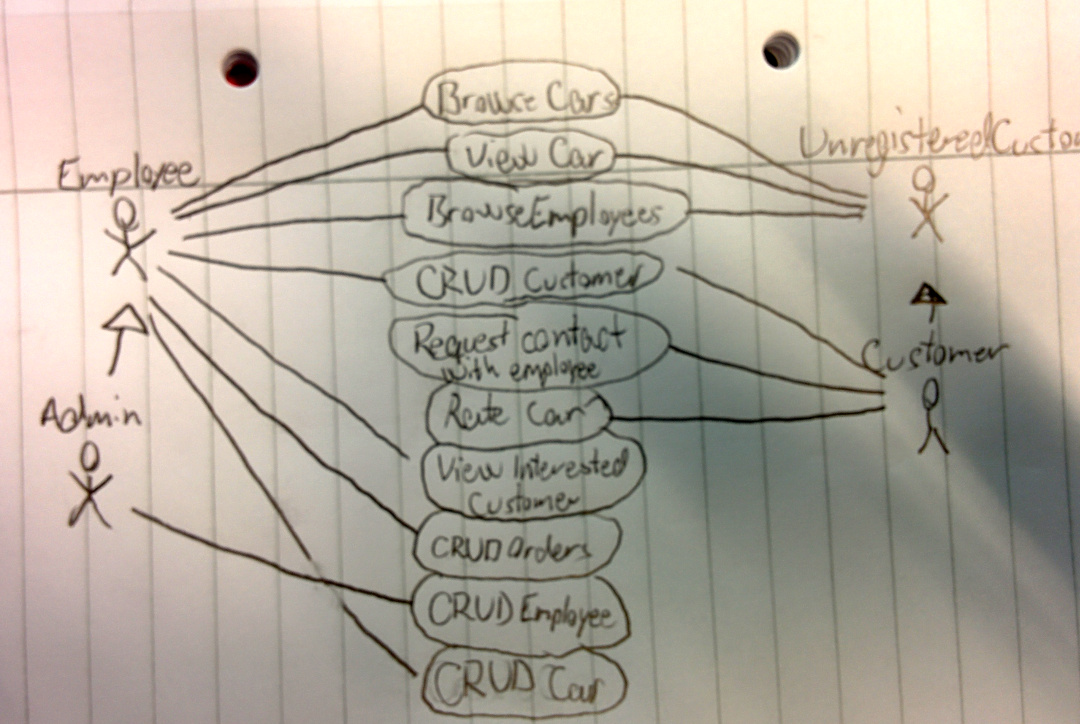
\includegraphics[scale=0.4]{Figures/UseCase-Model}\\
    \caption{The use case model - \texttt{Customer} inherits the unregistred customers cases, and the \texttt{Administrator} inherits from \texttt{Employee}}
  \label{fig:UseCaseModel}
\end{figure}

\newpage
\section{Use Cases}

\input{RAD-Part/UseCases/RAD-UseCase-CreateOrder}

\input{RAD-Part/UseCases/RAD-UseCase-CreateUser}

\input{RAD-Part/UseCases/RAD-UseCase-CreateCar}

\input{RAD-Part/UseCases/RAD-UseCase-ContactInterestedCustomer}

\input{RAD-Part/UseCases/RAD-UseCase-RequestEmployeeContact}

\section{Domain Object Models}

\begin{figure}[H]
	\centering
		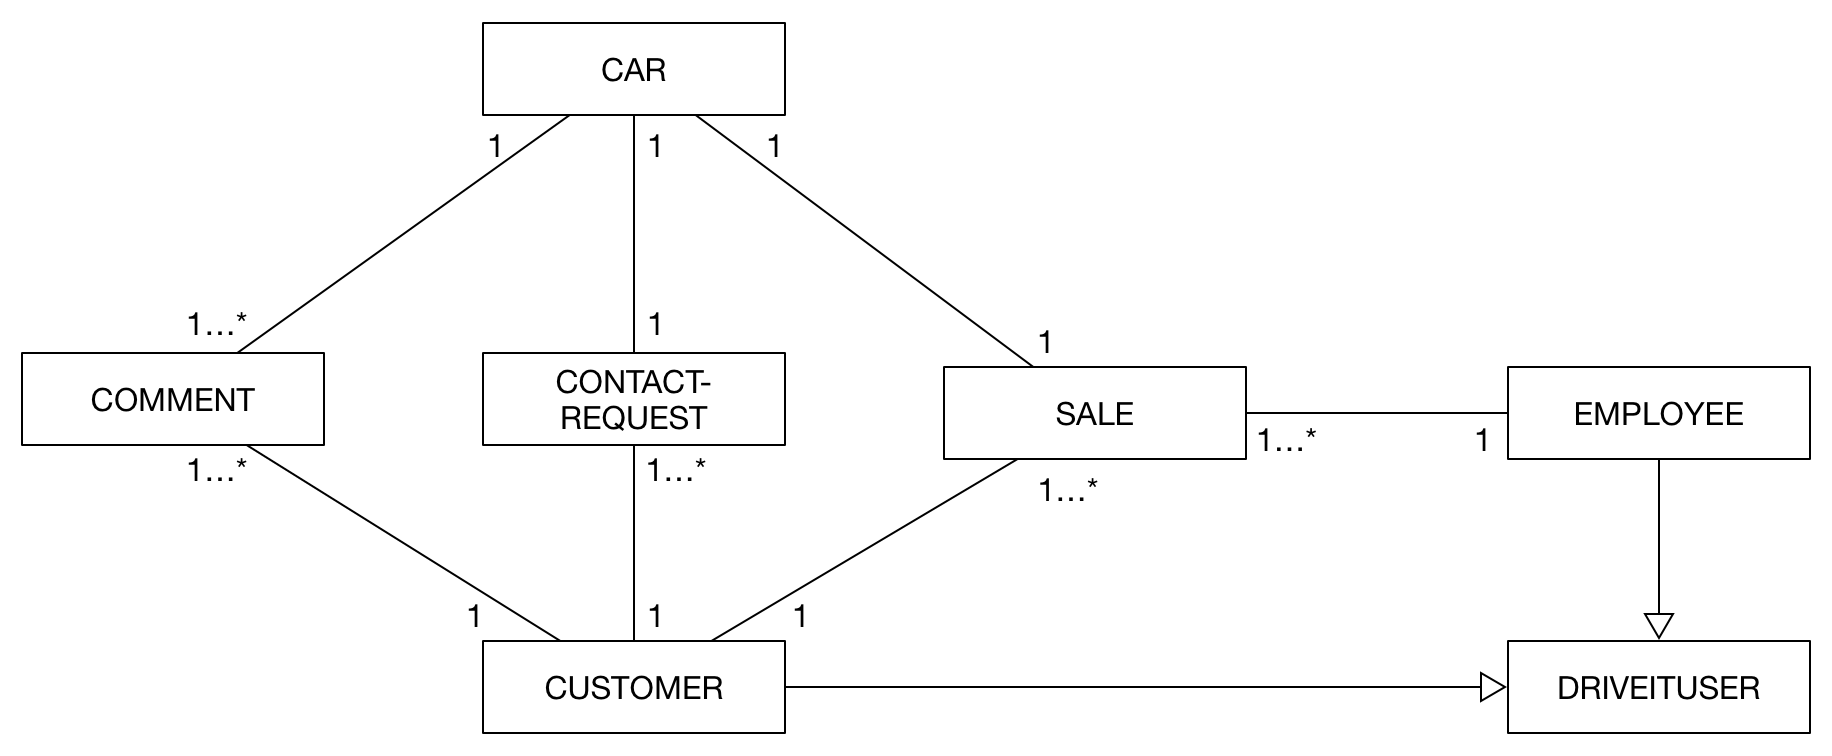
\includegraphics[scale=0.35]{Figures/DomainObjectModel}\\
		% place the figure in the Figures folder (located with the main file)
		% you need to fix the scale a few times to get it right, but latex does not compress so one can always zoom in to see details.
	\caption{The Domain Object Model of the \texttt{DriveIT System}.}
  \label{fig:DomainObjectModel}
  % label it something meanfull
\end{figure}

The \texttt{Car} object is a given used car that the car lot has purchased. A \texttt{Car} can have many or no \texttt{Comment}s. A \texttt{Comment} has only one \texttt{Customer}, but one \texttt{Customer} can create many \texttt{Comment}s.

A \texttt{Customer} can create many \texttt{Contact Request}s, but a given \texttt{Contact Request} can only come from one \texttt{Customer}.

When a  \texttt{Car} is purchased a \texttt{Sale} is created. A \texttt{Sale} can only have one \texttt{Customer}, one \texttt{Car} and one \texttt{Employee}.

One \texttt{Customer} can have many sales (if he/she buys many cars), but a given \texttt{Car} can only be sold once. An \texttt{Employee} can likewise have sold many cars.\\ 
An \texttt{Employee} represents an employee working at the used car lot, selling \texttt{Car}s to \texttt{Customer}s. The employee is referenced in a \texttt{Sale} when selling a \texttt{Car}.  

The \texttt{Admin} inherits from the \texttt{Employee} but has some special rights in the system (see Access Control).
\section{Dynamic Models}

\subsection{Use Case Sequence Diagrams}
\begin{figure}[h!]
	\centering
		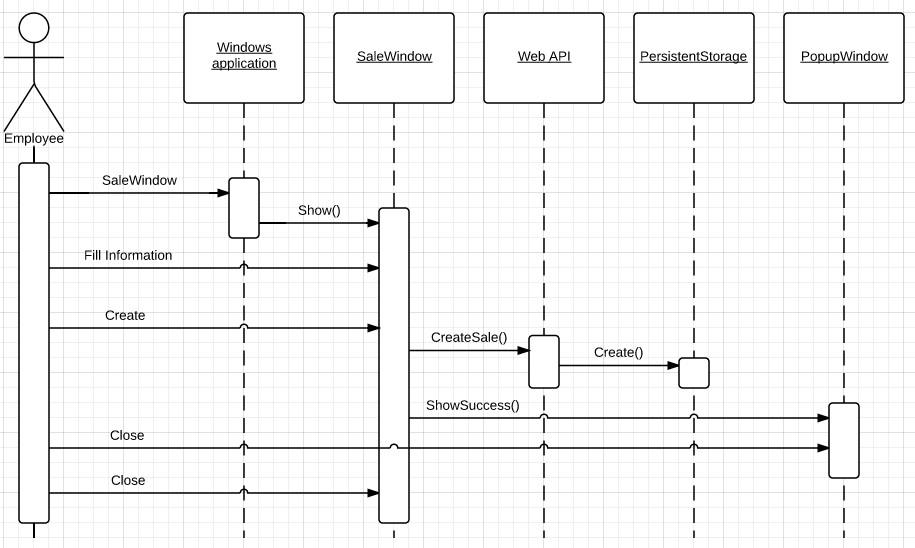
\includegraphics[scale=0.8]{Figures/SequenceDiagram-CreateOrder}\\
		% place the figure in the Figures folder (located with the main file)
		% you need to fix the scale a few times to get it right, but latex does not compress so one can always zoom in to see details.
	\caption{Sequence diagram of the CreateOrder use case.}
  \label{fig:SequenceDiagram-CreateOrder}
  % label it something meanfull
\end{figure}
\begin{figure}[h!]
	\centering
		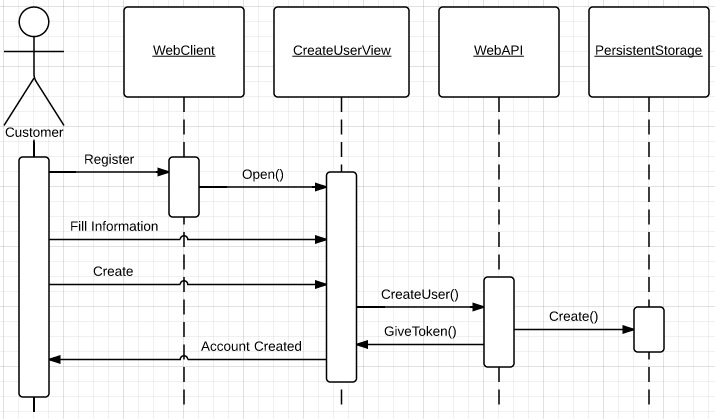
\includegraphics[scale=0.8]{Figures/SequenceDiagram-CreateUserAccount}\\
		% place the figure in the Figures folder (located with the main file)
		% you need to fix the scale a few times to get it right, but latex does not compress so one can always zoom in to see details.
	\caption{Sequence diagram of the CreateUserAccount use case.}
  \label{fig:SequenceDiagram-CreateUserAccount}
  % label it something meanfull
\end{figure}
\begin{figure}[h!]
	\centering
		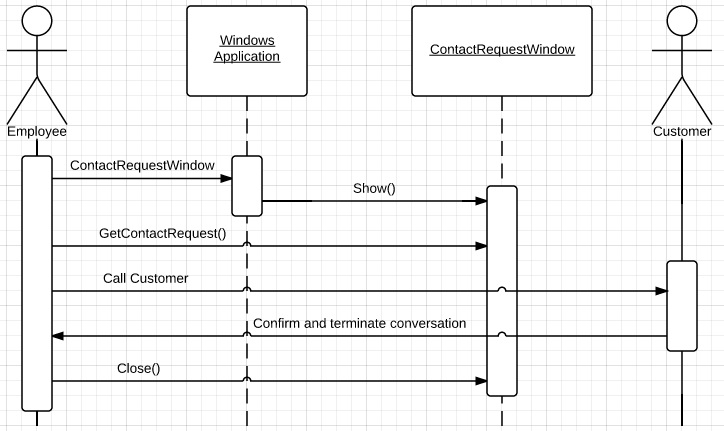
\includegraphics[scale=0.8]{Figures/SequenceDiagram-ContactInterestedCustomer}\\
		% place the figure in the Figures folder (located with the main file)
		% you need to fix the scale a few times to get it right, but latex does not compress so one can always zoom in to see details.
	\caption{Sequence diagram of the ContactInterestedCustomer use case.}
  \label{fig:SequenceDiagram-ContactInterestedCustomer}
  % label it something meanfull
\end{figure}
\begin{figure}[h!]
	\centering
		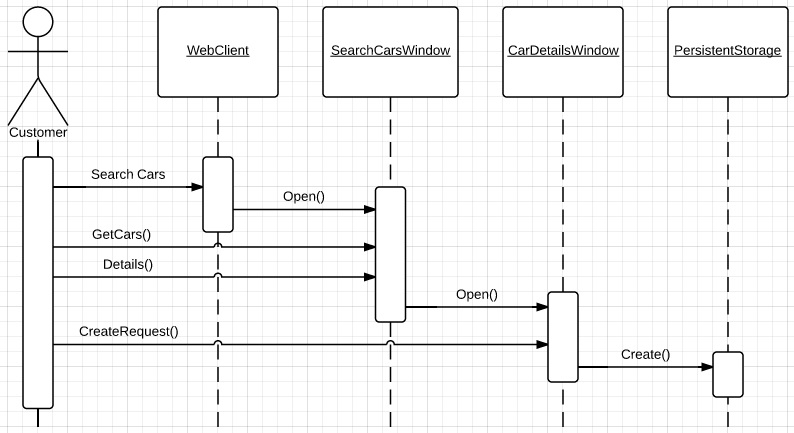
\includegraphics[scale=0.8]{Figures/SequenceDiagram-RequestEmployeeContact}\\
		% place the figure in the Figures folder (located with the main file)
		% you need to fix the scale a few times to get it right, but latex does not compress so one can always zoom in to see details.
	\caption{Sequence diagram of the RequestEmployeeContact use case.}
  \label{fig:SequenceDiagram-RequestEmployeeContact}
  % label it something meanfull
\end{figure}

\subsection{State Diagrams}
\begin{figure}[h!]
	\centering
		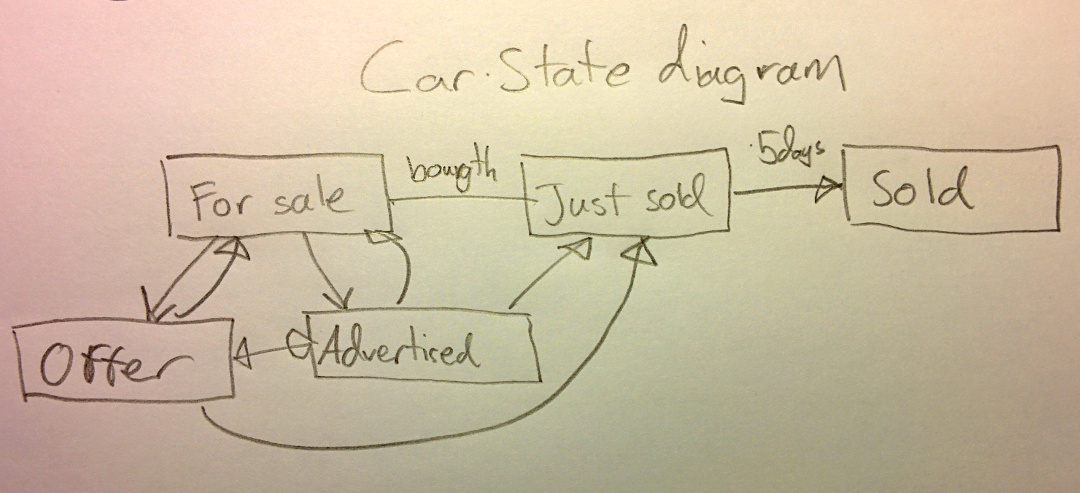
\includegraphics[scale=0.35]{Figures/StateDiagram-Car}\\
		% place the figure in the Figures folder (located with the main file)
		% you need to fix the scale a few times to get it right, but latex does not compress so one can always zoom in to see details.
	\caption{State diagram of the Car object}
  \label{fig:StateDiagram-Car}
  % label it something meanfull
\end{figure}
\begin{figure}[h!]
	\centering
		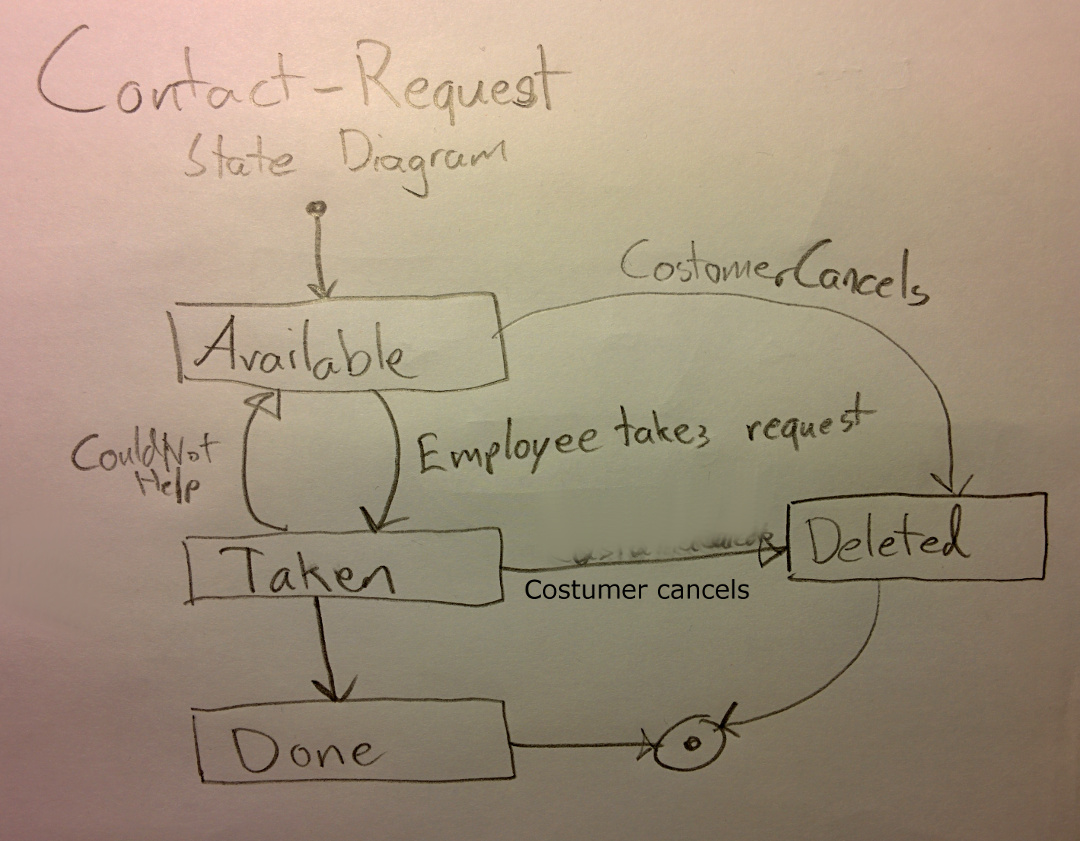
\includegraphics[scale=0.35]{Figures/StateDiagram-ContactRequest}\\
		% place the figure in the Figures folder (located with the main file)
		% you need to fix the scale a few times to get it right, but latex does not compress so one can always zoom in to see details.
	\caption{State diagram of the ContactRequest object}
  \label{fig:StateDiagram-ContactRequest}
  % label it something meanfull
\end{figure}
\subsection{User Interfaces}

\subsubsection{Windows Client}
The user interface was developed to have a native Windows look and feel from the beginning of the project. 
This means that anything superfluous has been removed, and that the content of the \texttt{DriveIT Windows Client} is in focus. 
The \texttt{Employee} needs to finish his/her task as quickly and efficiently as possible, which extra unnecessary user interface elements would hinder.
Motion has also been introduced in the interface in the form of user interface transitions when navigating menus. 
This all follows the Design Guidelines of Microsoft\footnote{\url{http://msdn.microsoft.com/library/windows/apps/hh781237.aspx}}.

The interface could have been more refined and made easier to use. The input fields for creating and updating entities could have fetched and parsed data dynamically, depending on the user context. 

When creating a \texttt{Sale} the "Car Id" field could present more meaningful selection options for the \texttt{Employee} e.g. model names with an attached ID. Currently the user has to know the ID in advance. \\
This goes for all entities.

\subsubsection{Prototyping}
A prototype was sketched and refined over the course of the project.\\
The final prototype can be seen below.\\

\textbf{Main Window:}
\begin{figure}[H]
	\centering
	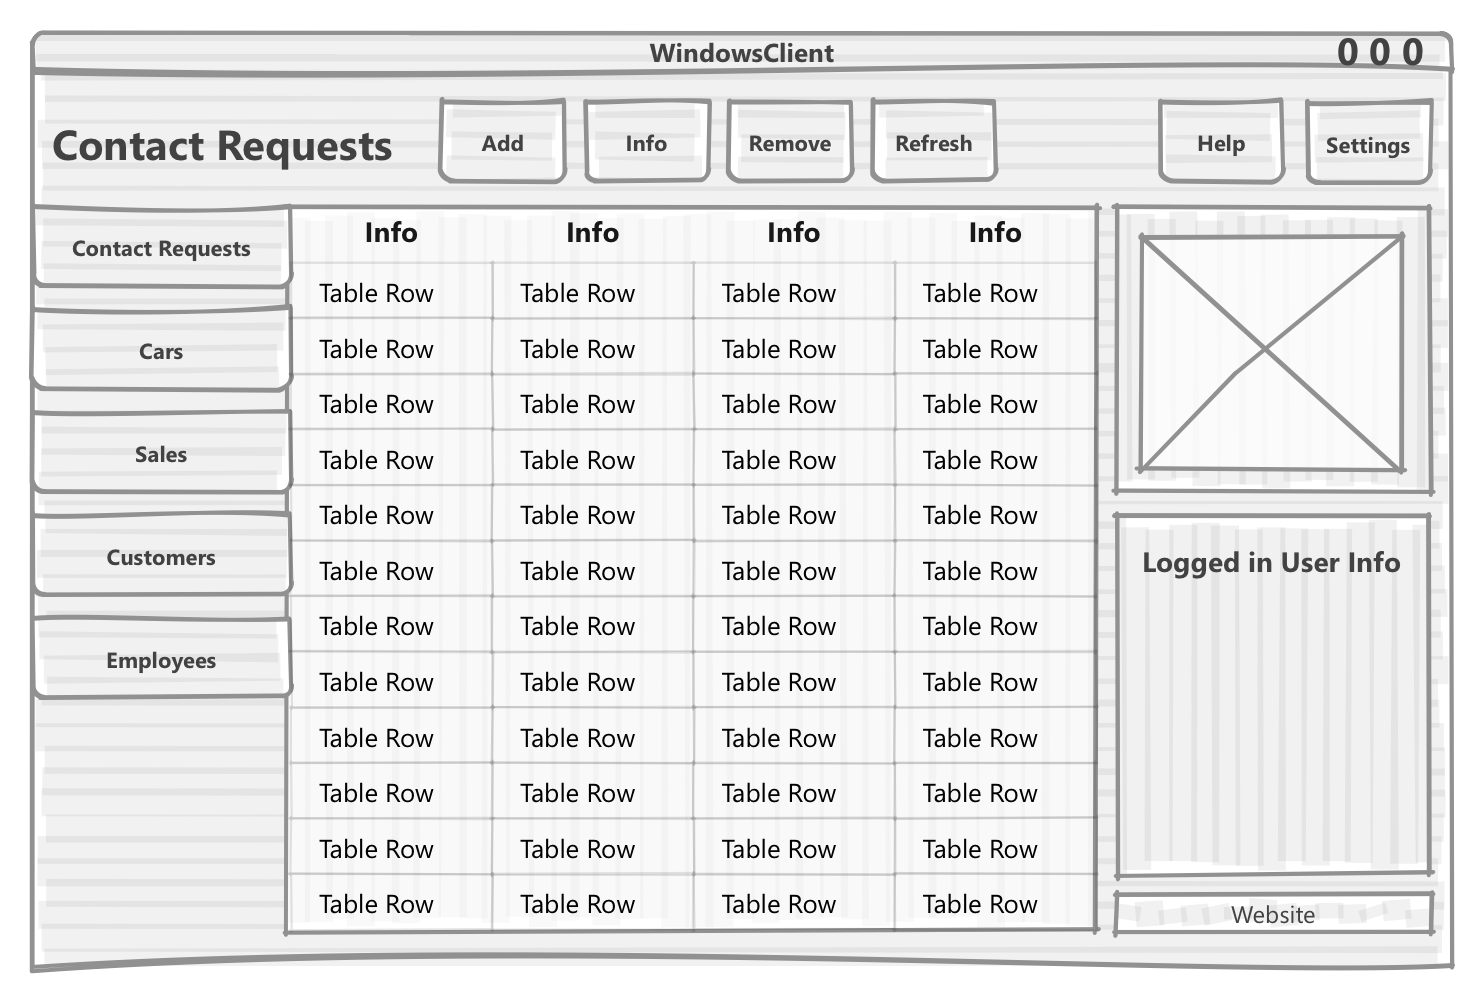
\includegraphics[scale=0.25]{Figures/UserInterface/WindowsMain}
	\caption{The Sketch of the Main Window of the Windows Client.}
	\label{fig:UserInterfaceWindowsMain}
\end{figure}
\textbf{Entity Windows:}
\begin{figure}[H]
	\centering
	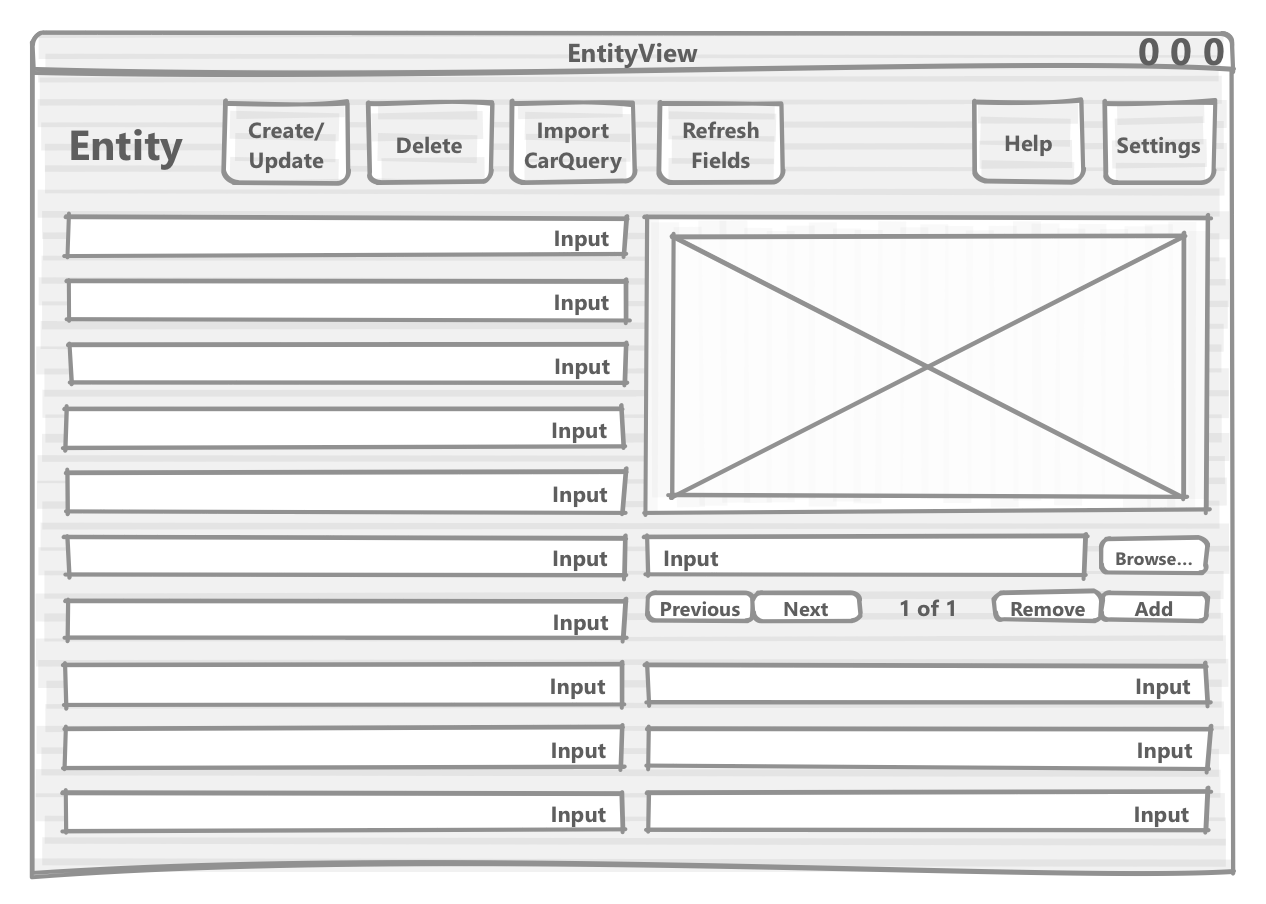
\includegraphics[scale=0.30]{Figures/UserInterface/EntityView}
	\caption{The Sketch of the Entity View of the Windows Client.}
	\label{fig:UserInterfaceEntityWindow}
\end{figure}

\part{System Design Document}
\chapter{Proposed Software Architecture}

\section{Design Goals}
\begin{enumerate}
\item Powerful and easy usability\\
The goal with the usability of the \texttt{DriveIT Windows client} is to give employees a powerful and easy to use tool to perform their work tasks. The gestalt laws are excellent examples on how to make a clean and simple user interface. The gestalt laws focuses on the placement of different GUI objects, such as buttons and text fields in a user interface, to make the interaction between user and user interface easy and painless for the user. By using the gestalt laws, we are able to make a clear distinction of which parts of the user interface that belongs to each other and thereby make it easier for the user to interact with the user interface. To give the Employees a powerful tool, the most frequently used tasks must be achievable quickly but with possible extensions to allow more advanced options. Thus making the usability fast while not dumping down on depth.\\\\
The goal with the usability of the \texttt{DriveIT Web client}, is to have a website which is simple and allows the user with only a few actions. This will decrease the possibility of confusion and therefore hopefully keep the users on the site. Gestalt laws should be used in the making the GUI such that it is easy for the user to see which functions maps together.

\item High Reliability\\
It is desired to create a reliable program that will prevent the user from losing progress made to the system, due to unexpected events, whereas an event could be a computer turn-off by accident or any other such similar things. How our system will be handling this, is by doing frequent auto-saving of the data, to a local data file, and then synchronize the auto-saved data with our data storage, to have an external backup of the data. Furthermore, every time the user commits anything, whereas this for example could be a new calendar entry, it will also be saved immediately to the local data file, and thereafter synchronize the local data file with the database. Force restarting should not be acceptable and most exceptions must be caught and handled during runtime. By doing the above mentioned, data loss will be kept to a minimum by limiting it to the user's current activity, should a failure occur.\\

\item Strong architecture with focus on extendability\\
When rolling out future updates for the system, a full re-installation of the program will be necessary. This is due to resources allocated to other more desired design goals.\\

\item Good documentation and Testing of the most important subsystems\\
The system will be tested before release, but in a limited way. As a full system test cannot be accomplished due to the time frame set for this systems development, a fully thorough testing will not be attainable, and we will therefore only focus on testing key components that are central parts of our system.
Documentation will be a central part of our system, as it is important to keep documentation of how the system works as a whole, and how the modules or subsystem works separately, and by making this documentation, it will be easier to extend our system by developers that have no knowledge about the system\\

\item High portability \\
To make sure that the system is easy to extend and scale, it will be build around a Web REST API that makes it easy to communicate with the system. This allows us to easily make apps for smart phones or other operating systems that supports and uses the DriveIT API. 

\item Easy and efficient implementation\\
The fact that the system will be developed and maintained in a popular and broadly used programming language such as C\#, assures a relatively painless implementations process. And since C\# uses the @.NET platform there are also a lot of well designed and highly maintained tools available, minimizing the implementation time and increasing the quality of the software.

\item TODO I don't really have any idea of what to write here? Just a quick discussion could help me,
\end{enumerate} 

\section{Overview}
This Software Design Document describes how the \texttt{DriveIT System} has been built.
This document describes the following:
\begin{itemize}
	\item Subsystem Decomposition
	\item Hardware and Software Mapping
	\item Persistent Data Management
	\item Access Control
	\item Global Software Control
	\item Boundary Conditions \&
	\item Persistent Data Management
\end{itemize}
The \texttt{DriveIT System} is primarily composed of five systems: 
A web client for customers to browse cars, a Windows client for employees to use, a Web API serving the clients data, a \texttt{CarQuery} system for fetching extra data about cars and a database system for storing and fetching data in a persistent storage system.
\section{Subsystem Decomposition}
The \texttt{DriveIT System} can be split into five main subsystems - the \texttt{DriveIT Windows Client}, \texttt{CarQuery}, \texttt{DriveIT Web Client}, \texttt{DriveIT Web API}, and \texttt{Persistent Storage} subsystems. 
These subsystems are described below. 

\subsection{The DriveIT System}
\begin{figure}[H]
	\centering
	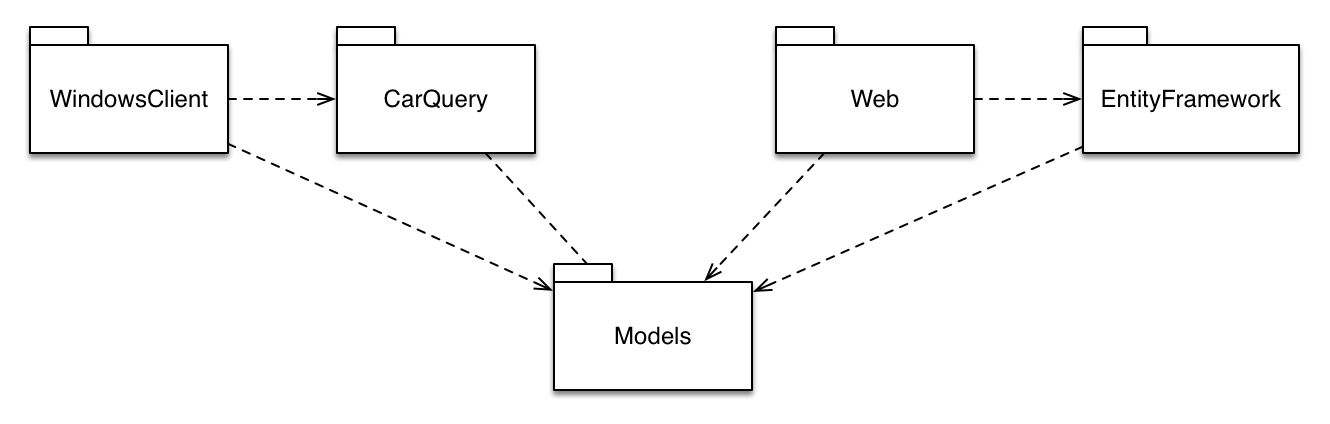
\includegraphics[width=\textwidth]{Figures/DriveITSubsystemDecomposition}\\
	\caption{Subsystems of the \texttt{DriveIT System}.}
\end{figure}

\subsection{Persistent Storage Subsystem} 
The Persistent Storage Subsystem manages storing and retrieving entity objects using the \textit{Entity Framework} and its serialisation functionality.\\
The serialised entities are stored in a \textit{Microsoft SQL Database} which is hosted on \textit{Microsoft Azure}. The subsystem provides the \texttt{DriveIT Web API} with deserialised entities, which uses the entities to provide the backend for other subsystems.\\
The subsystem supports retrieving all Entities of a given type, a specific entity using its unique ID, and retrieving an entity on its relation to other entities.
The Persistent Storage Subsystem consists of two classes and an interface (see figure \ref{fig:entityframeworksubsystem}). \texttt{EntityStorage} is the repository working on top of the \textit{Entity Framework} database layer, \texttt{DriveITContext}, providing the \texttt{IPersistentStorage} interface.

\begin{figure}[H]
	\centering
	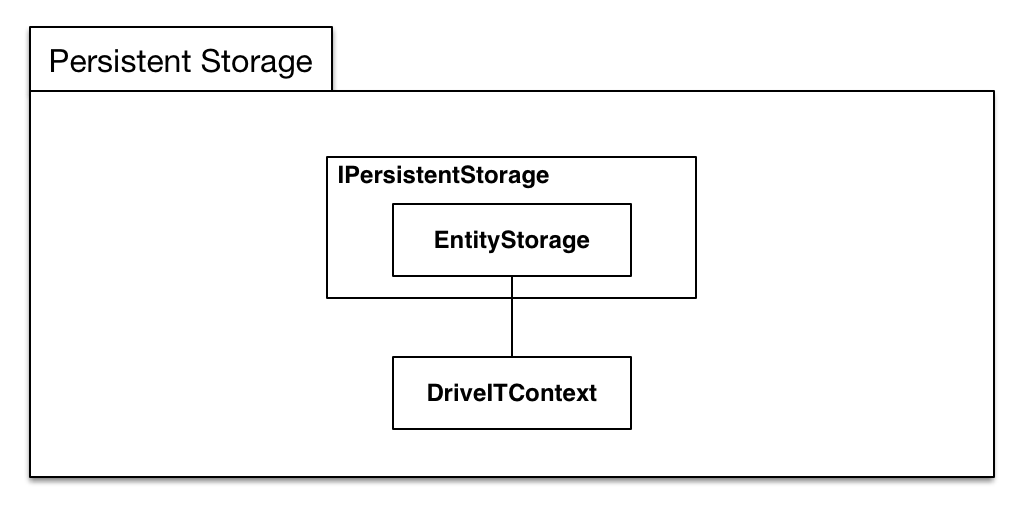
\includegraphics[width=\textwidth]{Figures/EntityFrameworkSubsystemDecomposition}
	\caption{Classes in the Persistent Storage Subsystem.}
	\label{fig:entityframeworksubsystem}
\end{figure}

\subsection{Web API}
The \texttt{DriveIT Web API}, which is built on \textit{ASP.NET Web API}\footnote{\url{http://www.asp.net/web-api}}, provides public communication with the \texttt{Persistent Storage} subsystem. This is done using specific URL routes. Furthermore it enforces authorisation so unauthorized users, and users with different user roles, only have limited access to the data of the \texttt{DriveIT System}.\\ 
Every table in the \texttt{Persistent Storage} subsystem must therefore be supported by the web API, although not every table is available to every user.\\
The \texttt{DriveIT Web API} is comprised of a series of modules for serialising the Model Entities into \texttt{JSON}\footnote{\url{http://en.wikipedia.org/wiki/JSON}} or \texttt{XML}\footnote{\url{http://en.wikipedia.org/wiki/XML}} and transferring these via a \texttt{REST} interface accessible using \texttt{HTTP}.\\
These modules are built into \textit{ASP.NET Web API}, and are not handled in our code.\\

The Web API consists of several controllers which uses a static class to translate \texttt{DTO's}\footnote{\url{http://en.wikipedia.org/wiki/Data_transfer_object}} into entities and vice versa. It is also the controllers that check for special cases, e.g. when a customer wants to update or delete a comment, and it is not allowed to change other \texttt{Customer}s' comments.

\subsection{Windows Client} 
\begin{figure}[H]
	\centering
	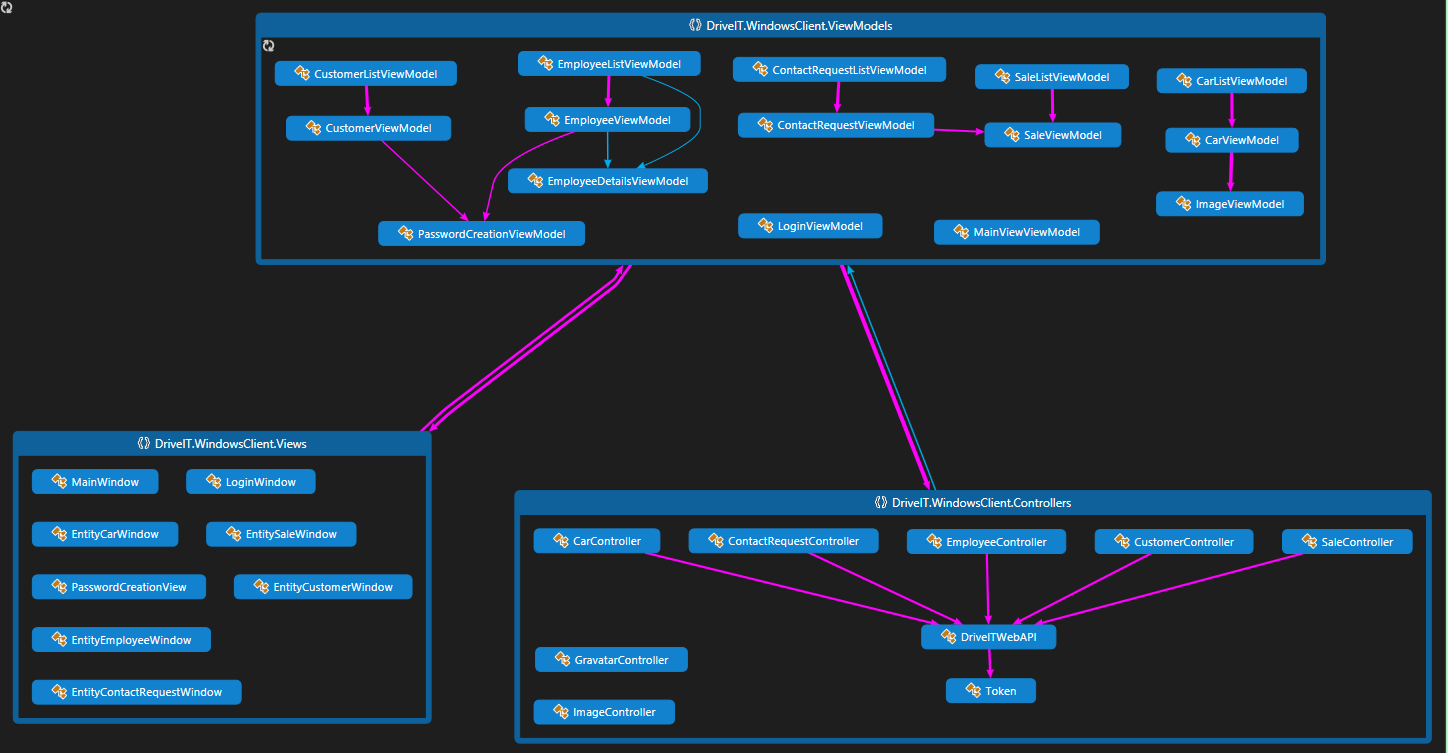
\includegraphics[width=\textwidth]{Figures/WindowsClientCodeMap}
	\caption{The Code Map of the Windows Client}
	\label{fig:WindowsClientCodeMapProper}
\end{figure}
The \texttt{DriveIT Windows Client} is used by the \texttt{Employee}s, to manipulate data in the \texttt{DriveIT System}. Depending on their role, \texttt{Employee} or \texttt{Administrator}, they can \textit{CRUD} all entities except for creating \texttt{ContactRequest}s.\\

The \texttt{Employee} signs in to the client with his or her email and password, and can then use the user interface to manipulate data in the \texttt{DriveIT System}.

The subsystem is made out of three main components: The \texttt{Views}, the \texttt{ViewModels} and the \texttt{Controllers}.

The \texttt{Views} package contains the user interface written in Windows Presentation Foundation (henceforth WPF). The \texttt{ViewModels} package contains the \texttt{ViewModel}s which hold data bound to the \texttt{View}s following Microsoft's \textit{Model View ViewModel} architectural pattern\footnote{\url{http://en.wikipedia.org/wiki/Model_View_ViewModel}}.

\texttt{ViewModel}s for entities are often created in the form of a \texttt{EntityListViewModel} and a \texttt{EntityViewModel}, but a few extra \texttt{ViewModel}s exists for additional \texttt{View}s such as the \texttt{LoginViewModel} and the \texttt{PasswordCreationViewModel}.

The \texttt{Controllers} package contains the \texttt{Controller}s which transforms data and sends and receives HTTP requests to and from the \texttt{DriveIT Web API}. Images are uploaded to \textit{Azure Blob Storage}. To provide \texttt{Employee}s and \texttt{Customer}s with profile pictures, a \texttt{GravatarController} exists to convert email strings into \textit{Gravatar}\footnote{\url{https://en.gravatar.com/}} profile URLs.

\subsection{Web Client}
The \texttt{DriveIT Web Client} is accessible through the Internet, where it is being used by non-registered and registered \texttt{Customer}s. The \texttt{DriveIT Web Client} is being used to search for \texttt{Car}s, that are up for sale in the \texttt{DriveIT System}.

The \texttt{DriveIT Web Client} allows the \texttt{Customer} to \textit{CRUD} \texttt{Comment}s if signed in. Otherwise \texttt{Comment}s can only be read.

It is also possible to \textit{create}, \textit{read} and \textit{delete} \texttt{ContactRequest}s and to read \texttt{Order}s and \texttt{Employee}s. A \texttt{Customer} is also able to \textit{read} and \textit{update} information regarding their own account.

It is possible to create an account on the web page with a non registered email.

The \texttt{DriveIT Web Client} is based on the \textit{ASP.NET MVC} framework\footnote{\url{http://www.asp.net/mvc}}, that is implementing the \textit{Model View Controller} design pattern (see section \ref{sec:MVC}).

\todo{rewrite}The subsystem is made of three components: Models, Views and Controllers. The views contains the user interface and is written in cshtml, which is a mix of C$\sharp$ and HTML code. The models contains lists of database records and the controllers are responsible for giving the models, filled with database records, to the views, for them to display the data in the model.

\subsection{CarQuery} 
This subsystem is a collection of classes that enable the the \texttt{DriveIT Windows Client} to fill out missing information about cars, using the \textit{CarQuery API}.\\
The subsystem is used by an \texttt{Employee} when creating or updating a \texttt{Car}. The subsystem consists of a \textit{JSON} deserialiser that communicates with the \textit{CarQuery API} and another class that receives a \texttt{Car} object and fills out the missing attributes using the deserialised \textit{JSON} data.

An \texttt{Employee} fills out the known information about the \texttt{Car} and the \texttt{CarQuery} subsystem then creates its query on the \textit{CarQuery API}.

Only the \texttt{CarQuery} static class is publicly accessible. As seen in figure \ref{fig:carquerysubsystem} it uses a \texttt{JSONWrapper} to receive data from the \textit{CarQuery API} and deserialises it into a \texttt{Trims} object which is an array of \texttt{Trim} objects holding the actual \texttt{Car} data.
\begin{figure}[H]
	\centering
	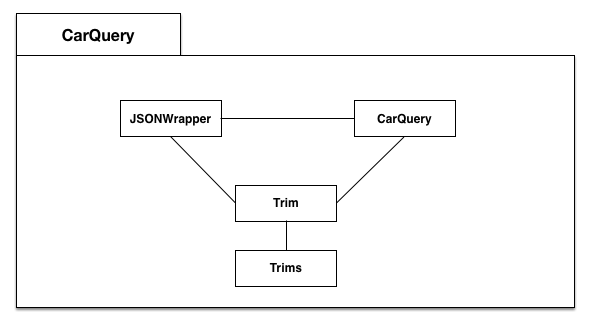
\includegraphics[width=\textwidth]{Figures/CarQuerySubsystemDecomposition}\\
	\caption{Classes of the \texttt{CarQuery} Subsystem.}
	\label{fig:carquerysubsystem}
\end{figure}
\section{Hardware and Software Mapping}
As figure \ref{fig:Hardware-Software-Mapping} shows, we want to run the DriveIT subsystems on the following hardware:\\

The Persistence, \texttt{DriveIT Web API} and \texttt{DriveIT Web Client} subsystems will be hosted on a web server running ASP.NET. We have chosen \texttt{Microsoft Azure} as our host.

The \texttt{DriveIT Web API} uses Persistence module internally to contact the \texttt{Microsoft SQL Server} that runs behind the \texttt{Entity Framework}.

The \texttt{DriveIT Web Client} is accessed through a modern web browser using HTTP. It uses the \texttt{DriveIT Web API} internally, and as they are located in the same project, they can be hosted at the same address on \texttt{Microsoft Azure}.\\

The \texttt{DriveIT Windows Client} runs on .NET 4.5 and uses the \texttt{CarQuery} subsystem, which helps \texttt{Employee}s fill out missing information about cars. The \texttt{DriveIT Windows Client} communicates with the \texttt{DriveIT Web API} subsystem through HTTP. The content of the HTTP-requests and responses are Json objects when data transfer is needed.

\begin{figure}[H]
	\centering
	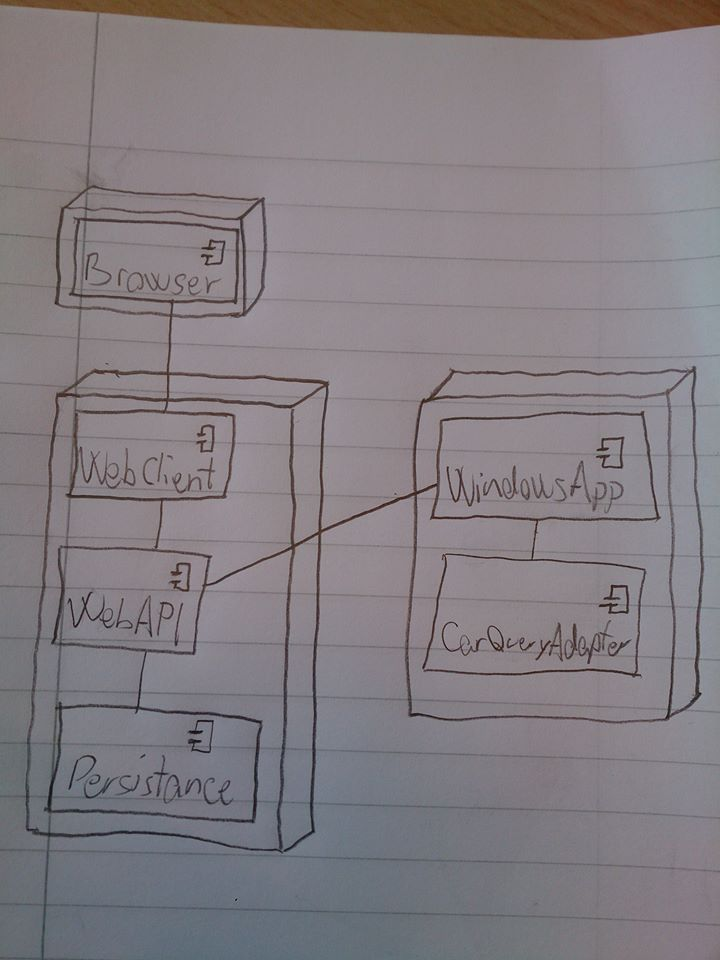
\includegraphics[width=\textwidth]{Figures/HardwareSoftwareMapping}
	\caption{Hardware software mapping of the entire system.}
	\label{fig:Hardware-Software-Mapping}
\end{figure}
\section{Persistant Data Management}
Data of most entities in the \texttt{DriveIT System} needs to be stored persistently to avoid data loss if the system crashes and ensure that users can expect to resume work from the point where they last left.
The EntityFramework sub system stores this data using an SQL database hosted online. 
It stores the following entities:
\begin{itemize}
	\item \textbf{Car:} Representing a used car. Cars are read, modified and deleted in every sub system in the \texttt{DriveIT System}.\\
	Cars have many attributes, all describing the properties of the car. Cars are referenced in many other entities in the storage system, but do not reference other entities themselves.\\
	\item \textbf{Customer:} Representing a potential buyer of cars. Customers are read by some parts of the system, but only modified and deleted in certain authorized instances. \\
	Customers have few attributes describing the person acting as the customer. Customers are referenced in some entities in the storage system, but do not reference other entities themselves.
	\item \textbf{Employee:} Representing a salesman of cars. Employees are read by some parts of the system, but only modified and deleted in certain authorized instances. \\
	Employees have few attributes describing the person selling cars. Employees are referenced in some entities in the storage system, but do not reference other entities themselves.
	\item \textbf{Sale:} Representing a sale of a car. Sales are read by some parts of the system, but only modified and deleted in certain authorized instances. \\
	Sales have few attributes describing the specific sale, but mainly reference other entities. A given sale references an \texttt{Employee}, a \texttt{Car} and a \texttt{Customer}.
	\item \textbf{Comment:} Representing a comment on a car. Comments are read by some parts of the system, but only modified and deleted in certain authorized instances. \\
	Comments have few attributes describing the specific comment, but mainly reference other entities. A given comment references a \texttt{Car} and a \texttt{Customer}.
	\item \textbf{ContactRequest:} Representing a request for contact by an \texttt{Employee} about a \texttt{Car}. ContactRequests are read by few parts of the system and only modified and deleted in certain authorized instances. \\
	ContactRequests have one attribute describing the specific request, but mainly reference other entities. A given ContactRequest references a \texttt{Car} , an \texttt{Employee} and a \texttt{Customer}.
\begin{figure}[h!]
	\centering
		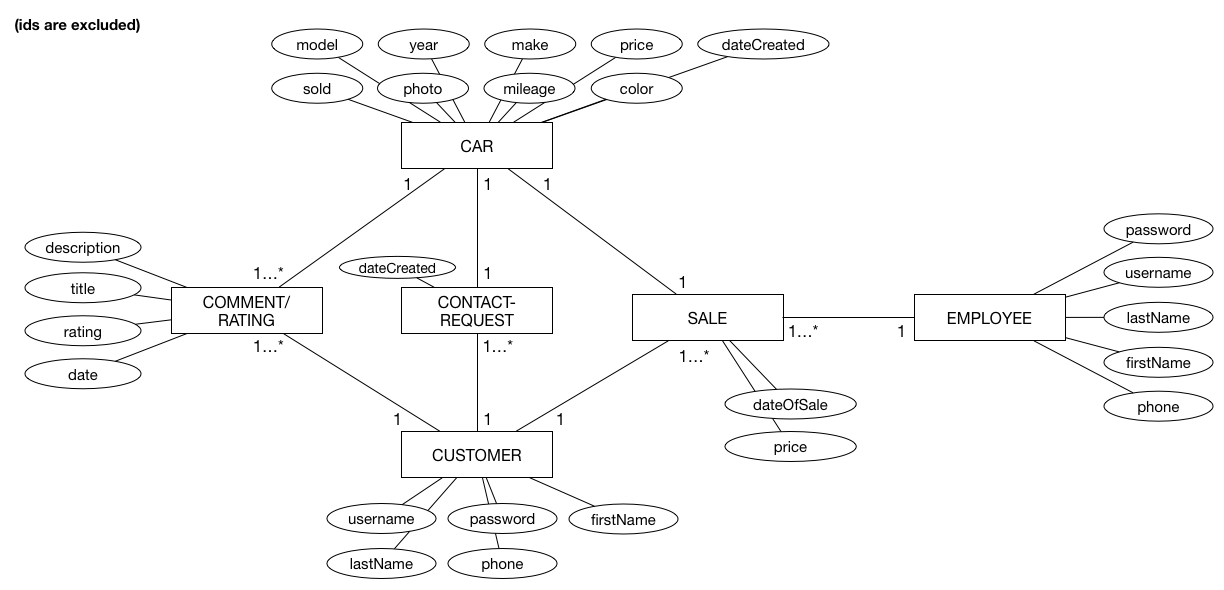
\includegraphics[scale=0.30]{Figures/PersistentDataModel}\\
		% place the figure in the Figures folder (located with the main file)
		% you need to fix the scale a few times to get it right, but latex does not compress so one can always zoom in to see details.
	\caption{The Persistent Data Model.}
\end{figure}
\section{Access Control and Security}

\todo{Check that it matches the program/api}
\textbf{Access Matrix for DriveIT System}

\begin{tabular}{|l|*{6}{c|}}\hline
\backslashbox{\miniscule\textbf{Actors}}{\miniscule\textbf{Entities}} & \miniscule\textbf{Car} & \miniscule\textbf{Comment} & \miniscule\textbf{ContactRequest} & \miniscule\textbf{Customer} & \miniscule\textbf{Employee} & \miniscule\textbf{Sale} \\\hline

\miniscule\textbf{Non-registered user} & \miniscule read & \miniscule read && \miniscule create & \miniscule read & \miniscule\\\hline

\miniscule\textbf{Customer} & \miniscule read & \miniscule create & \miniscule create & \miniscule read & \miniscule read & \miniscule read\\
	&& \miniscule read & \miniscule read & \miniscule update &&\\
	&& \miniscule update & \miniscule delete &&& \\
	&& \miniscule delete &&&&\\\hline

\miniscule\textbf{Employee} & \miniscule create & \miniscule read & \miniscule read & \miniscule create & \miniscule read & \miniscule create \\
	& \miniscule read && \miniscule update & \miniscule read && \miniscule read\\
	& \miniscule update && \miniscule delete & \miniscule update && \miniscule update\\
	& \miniscule delete &&&&& \miniscule delete\\\hline

\miniscule\textbf{Administrator} & \miniscule create & \miniscule read & \miniscule read & \miniscule create & \miniscule create & \miniscule create\\
	& \miniscule read & \miniscule delete & \miniscule update & \miniscule read & \miniscule read & \miniscule read\\
	& \miniscule update && \miniscule delete & \miniscule update & \miniscule update & \miniscule update\\
	& \miniscule delete &&& \miniscule delete & \miniscule delete & \miniscule delete\\\hline

\end{tabular}\\\\

Due to the fact that the DriveIT System is available for many users, it is necessary to keep track of which users may have access to specific resources in our system. To keep track of which users got access to which resources, it is necessary to check each user at login, through authentication, to confirm which resources they can access.\\

In our system, a non-registered user (a person accessing the DriveIT homepage without logging in) should be restricted to only be able to search for cars, get a list of employees and create a new user on the homepage.\\

The customer is able to access more on the DriveIT homepage than a non-registered user. The customer is able to access the same information as a non-registered user, but are also able to look through his or her own orders, and also able to create, update or delete his or her own comments on cars.\\

The employee is able to create, update or delete cars, and search for cars. The employee is also able to create a new user (if a person calls the \todo{company using DriveIT?}company using DriveIT for help), get information about a specific user and update a user by request of a customer. The employee is also able to create an order, see the orders of a specific customer, update an order and delete an order. The employee should also be able to get a list of employees, if it is needed in any case.\\

Administrators of the system can do everything the employee can, but also create, update and delete other employees and administrators.

There is a bug in the DriveIT Web Client which means that employees and administrators can login and create comments and contact requests as well. They cannot manage other peoples comments and contact requests though, and also they cannot see own orders and contact requests through the managing menu. Information about employees and administrators cannot be changed through the Web Client, as it was not meant to support this feature.
\section{Global Software Control}

The flow of the \texttt{DriveIT System} would be a \textit{Procedure-driven control}\footnote{{Object-Oriented Sofware Engineering - 3rd Edition - 2009 - page 275}}\todo{find out year of book}, and the reason for this, is that the program will follow specific procedures, depending on how the \texttt{Customer}/\texttt{Employee} is interacting with the system.\\

Upon starting the system, the \texttt{Customer} will be presented with the main view of the system. It is not required to log into the system to use it. The \texttt{Customer} can freely navigate through the database searching for cars given the search criteria. Only when the \texttt{Customer} wishes to be contacted about a Car, a login will be prompted.\\ 

This differs a bit for the \texttt{Employee} as their usage of the system is different. An \texttt{Employee} has tasks which require a higher access level, that are not available for a \texttt{Customer}. Therefore an \texttt{Employee} will log in upon starting up the system, and hereby verify the authorization level.\\

For logging in, the \texttt{LoginViewModel} of our \texttt{ViewModel Subsystem} will use the information entered into our login view to authenticate the information, and if the authentication through the \texttt{EmployeeController} of the \texttt{Controller Subsystem} is a success, the \texttt{Persistence Subsystem} will access the information belonging to the \texttt{Customer}/\texttt{Employee}, and our \texttt{ViewModel Subsystem} will then observe the \texttt{Persistence Subsystem} and update its state, whereafter the \texttt{DriveITMainView}, from our \texttt{View Subsystem}, will be initialized and show the data received from the database.\\

The \texttt{Customer} can now interact with the sytem in multiple ways. For instance, the \texttt{Customer} can view the cars they are interested in. This task is handled by the \texttt{Controller Subsystem}, which updates the state of the \texttt{Model Subsystem} which is then reflected in the \texttt{DriveITMainView}, which will register the activity of the \texttt{Customer}, update the state of the Model and then load it into the DriveITSystemView. In the background, new activity will be stored in the database, as the \texttt{Customer} is still using the system. If a change is commited, the Model will update its own state, whereafter the \texttt{DriveITMainView} will be updated by the \texttt{ViewModel Subsystem}.\\

On the other hand an \texttt{Employee} will have the main task of handling requests for contact by a \texttt{Customer}. Anybody with \texttt{Employee} authentication, will have a shared `forum', where they can view a list of \texttt{Users} who are interested in cars/contact from an \texttt{Employee}. An \texttt{Employee} can now drag one of these requests into their own workfield and hereby claim a task. The same way as the task for a \texttt{Customer} above, the task will be  handled by the \texttt{Controller Subsystem}, which updates the state of the \texttt{ViewModel Subsystem} which is then reflected in the \texttt{DriveITMainView}. This will register the activity of the \texttt{Employee}, update the state of the Model and then load it into the \texttt{DriveITMainView}. In the background, new activity will be stored in the database, as the \texttt{Employee} is still using the system. If a change is commited, the Model will update its own state, whereafter the \texttt{DriveITMainView} will be updated by the  \texttt{ViewController Subsystem}.\\
\section{Boundary Conditions}
\subsection{Service Boundary Condition}
For the \texttt{DriveIT Web Client} and the \texttt{DriveIT Windows Client} to be initiated the \texttt{DriveIT Web API} must have been initialised otherwise all functionality will be unavailable. 

Furthermore the \texttt{DriveIT Web API} must run constantly to allow the clients to persist and retrieve data.

\subsection{Subsystem Boundary Condition}
\subsubsection{DriveIT Web Client}
On initialisation of the \texttt{DriveIT Web Client} all controllers are configured to map to certain routes. Furthermore \textit{OWIN}\footnote{\url{http://owin.org}} configured for the \texttt{DriveIT Web Client}. This is all done automatically by \textit{ASP.NET} and \textit{OWIN}. 

Every time a page is loaded the data shown in the view is read from the \texttt{DriveIT Web API}, thereby synchronising data.

Exceptions which are not caught and handled, will display a generic status message, but will not crash the server.

No actions are currently performed at shutdown.

\subsubsection{DriveIT Windows Client}
On initialisation of the \texttt{DriveIT Windows Client} an \texttt{Employee} must sign in with valid account in the \texttt{LoginView}. This initialises the static class \texttt{DriveITWebAPI} such that an connection to the \texttt{DriveIT Web API} is can be established when needed.

To synchronise with the \texttt{DriveIT Web API}, the \texttt{DriveIT Windows Client} updates data each time a list-\texttt{View} changes.

The \texttt{DriveIT Windows Client} handles exceptions by displaying a error message to the user in the \texttt{View} where the error originated. This is displayed in a status label, mentioning which action went wrong.

On shutdown the objects of the \texttt{DriveIT Windows Client} are disposed by the \textit{CLR}\footnote{\url{http://msdn.microsoft.com/en-us/library/8bs2ecf4\%28v=vs.110\%29.aspx}}. No further actions are performed.
\chapter{Sub System Services}
\part{Object Design Document}
\chapter{Object Design and Patterns}
\section{Object Design}

\subsection{Persistent Storage}

\subsubsection{Reuse}
The \texttt{EntitiyStorage} class is very specific for the \texttt{DriveIT System} since it only deals with creating, reading, updating and deleting \texttt{DriveIT} entities. It therefore does not provide any major re-usability for other purposes than this. 

Adding re-usability could be accomplished by using generics (supported by the C$\sharp$ language), which would allow the system to create, read, update and delete any input entity, provided it was supported by the given \texttt{DbContext}. This would allow for greater extensibility and easier code maintenance.

\subsubsection{Inheritance}
The \texttt{DriveITContext} extends an \texttt{IdentityDbContext} which provides the built in functionality for handling user logins and different user roles, which is used for the login- and access control functionality of the \texttt{DriveIT System}.
The \texttt{IdentityDbContext} in turn extends a \texttt{DbContext} which enables \texttt{Entity Framework} to save the User entities (along with every other \texttt{DriveIT} entity) in the underlying Microsoft SQL database.

\subsubsection{Encapsulation}
Encapsulation has been a high priority during development of the \texttt{DriveIT System}. 

Keeping functionality of different sub systems encapsulated has helped debugging and refactoring. Extensibility is also made easier in the future.

Encapsulation has been used in the \texttt{Persistent Storage} system in methods dealing with retrieving, editing and deleting entities. Methods generally have few side effects and only do not keep references to others classes after performing their task.

A design choice in implementing the methods were to only keep a \texttt{DriveITContext} (which inherits from \texttt{DbContext}) in memory for a short amount of time to ensure that the context only fulfilled its purpose in dealing with the entities and then was discarded.

Updating entities requires copying all attributes of the entity which is done in separate methods without side effects.

\subsection{CarQuery}

\subsubsection{Reuse}
The \texttt{JSONWrapper} of the \texttt{CarQuery} sub system is written using generics, which enables using any object and URL as input for getting and deserialising aserialised JSON object, provided that the properties of the input object match the received JSON data. 
The class is only used by the \texttt{CarQuery} system, though. This functionality could be used by other classes in the system for communicating with e.g. the \texttt{DriveIT Web API}. 
Having a generic method for dealing with filling out properties instead of a specific \texttt{Car}-only method would also have benefited reuse of the system.

\subsubsection{Encapsulation}
The functionality of the \texttt{CarQuery} sub system is implemented using few static classes with few methods dealing with small tasks. The classes have been made static due to the fact that their functionality has a "use and forget"-feel to them. 

The sub system is used in short periods of time and only has one purpose: getting \texttt{Car} data. Therefore no object needs to be kept in memory, data should just be deserialised and added to a \texttt{Car}. The entire \texttt{CarQuery} sub system is therefore made up of static functionality.
\section{Interfaces}

\subsection{Persistent Storage}
The \texttt{PersistentStorage} sub system provides an interface \texttt{IPersistenStorage}, which gives access to creating, reading, updating and deleting \texttt{DriveIT} entities. 
\subsubsection{Implementors, Extenders \& Users}
The IPersistentStorage has an implementor, EntityStorage, which in turn uses a DriveITContext to accomplish its tasks. 

\subsubsection{Visibility}
The 
\section{Design Patterns}
\subsection{Model View ViewModel Pattern}
\begin{figure}[H]
	\centering
	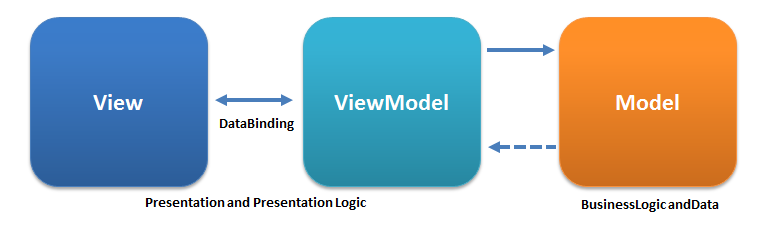
\includegraphics[width=\textwidth]{Figures/WebImages/MVVMPattern}\\
	\caption{The Model View ViewModel Pattern}
	\label{fig:MVVMPattern}
\end{figure}
The \texttt{DriveIT Windows Client} uses the \textit{Model View ViewModel}\footnote{\url{http://en.wikipedia.org/wiki/Model\_View\_ViewModel}} (hereafter \textit{MVVM}) architectural pattern which tries to ensure a clear separation between the \textit{Model} and the \textit{View}. The pattern derives from both the \textit{Model View Controller} pattern and the \textit{Presentation Model} design pattern. Therefore it has some of the same attributes. By using the \textit{MVVM} pattern we created a more testable and easier expandable application.

Furthermore we used \textit{Microsoft Blend}'s\footnote{\url{http://en.wikipedia.org/wiki/Microsoft_Blend}} built in \textit{Actions}\footnote{\url{http://blogs.msdn.com/b/expression/archive/2009/03/23/an-introduction-to-behaviors-triggers-and-actions.aspx}} to encapsulate calls and commands from the \texttt{View} such that \texttt{View} elements would be sent to the \texttt{ViewModel}. These actions are implemented to ensure low coupling.\\

A built-in part of \textit{MVVM} is a version of the \textit{Observer-Pattern}\footnote{\url{http://en.wikipedia.org/wiki/Observer_pattern}}. This is done by creating data-bindings between the \texttt{View} and their \texttt{ViewModel}. In \textit{WPF} this is achieved by having the \texttt{ViewModel}s implement the interface \texttt{INotifyPropertyChanged} which will notify the \texttt{View} when the \texttt{ViewModel} has changed. By using this interface the \texttt{ViewModel} knows nothing of the \texttt{View} and cannot directly change its attributes.

\subsection{Adapter Pattern}
The \textit{Adapter pattern} allows the developer to encapsulate methods and properties of an object in an "Adapter" class. Since the \texttt{DriveIT Windows Client} uses the \textit{MVVM} design pattern, and the \texttt{DriveIT Web API} uses \textit{DTO}s to send and receive data, and \textit{DTO}s are only meant to transfer data, an Adapter Pattern fits perfectly. Almost all single entitiy \texttt{ViewModel}s in the \texttt{DriveIT.WindowsClient.ViewModels} namespace function as adapters for their corresponding \textit{DTO}. E.g the \texttt{CarViewModel} class is an adapter for the \texttt{CarDto} class.\\ 

This implementation provides the \texttt{DriveIT Windows Client} with an easy way to manipulate data, while still retaining the data structure such that entities can be created, read, updated, and deleted over the \texttt{DriveIT Web API} without the having to convert client classes to API classes.

\subsection{Model View Controller Pattern}
\label{sec:MVC}
\begin{figure}[H]
	\centering
	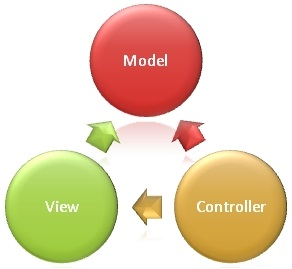
\includegraphics[width=\textwidth]{Figures/WebImages/MVCPattern}\\
	\caption{The Model View Controller Pattern}
	\label{fig:MVCPattern}
\end{figure}
The \texttt{DriveIT Web Client} uses the \textit{Model View Controller}\footnote{\url{http://www.w3schools.com/aspnet/mvc_intro.asp}} (henceforth \textit{MVC}) architectural pattern, which is making a separation of the business logic, the \textit{Model}, and the input control, the \textit{Controller}, from the display logic, \textit{View}.

The model is the part of the application that wil be handling all the logic for the application data. The models are being used to store data from the dabatase.
The view is the part of the application that will be handling the representation of the data. Most often, this data will be given by the model.
The controller is the part of the application that will be handling the user interaction with the \texttt{DriveIT Web Client}. The controllers reads the user input and updates the model's state.

The MVC pattern allows for seperation of the model, view and the controller classes, such that their individual purposes are clearly distinct from each other. This means that different developers are able to work on each of the individual parts of the MVC pattern, E.g we are able to work on the view without depending on the business logic (model) or the input (controller). By making this distinction between different parts of the MVC pattern, it also makes it easier to test our \texttt{DriveIT Web Client} application, and remain a good data-structure throughout the development of our Web Client.

\todo{Write more specific about how we have implemented it in our system.}

\subsection{Façade Pattern}
The facade design pattern is used several times in the \texttt{DriveIT System}.
The \texttt{Persistent Storage} sub system uses a facade pattern do hide the internal sub systems that accomplish the functionality defined in the \texttt{IPersistentStorage} interface.

The \texttt{DriveITContext} defined in the sub system is used by an implementer, \texttt{EntityStorage}, on the interface, but is hidden for users of the interface. 

\begin{figure}[H]
	\centering
	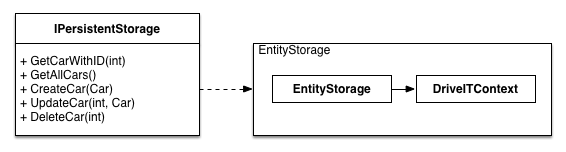
\includegraphics[scale=0.6]{Figures/FacadePatternPersistentStorage}\\
	% place the figure in the Figures folder (located with the main file)
	% you need to fix the scale a few times to get it right, but latex does not compress so one can always zoom in to see details.
	\caption{The Facade Pattern of IPersistentStorage.}
	\label{fig:The Facade Pattern of IPersistentStorage.}
	% label it something meanfull
\end{figure}

\begin{figure}[H]
	\centering
	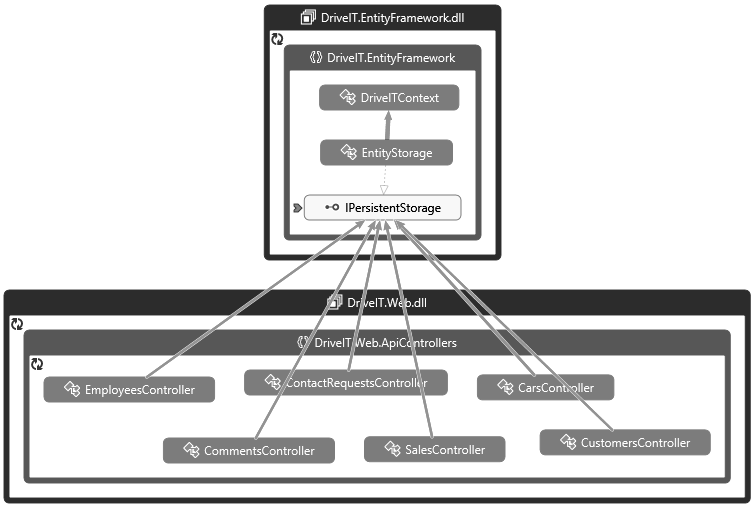
\includegraphics[scale=0.6]{Figures/FacadeKindOfPattern}\\
	% place the figure in the Figures folder (located with the main file)
	% you need to fix the scale a few times to get it right, but latex does not compress so one can always zoom in to see details.
	\caption{The Facade Pattern Used by the \texttt{DriveIT Web API}.}
	\label{fig:The Facade Pattern Used by the DriveIT Web API.}
	% label it something meanfull
\end{figure}

\part{Test Document}
\chapter{Test Plan and Results}
\section{Overall Test Approach}
One of the non-functional requirements and design goals of the \texttt{DriveIT} system was to test critical sections of the system.

This has been accomplished by using a bottom-up testing approach. 
The deeper layers of the system providing data have been unit tested. Other subsystems of the \texttt{DriveIT System} building on top of these unit testes subsystems have been integration or system tested. 

Trusting that the lower layers of the system function correctly enables that these can be used directly for integration testing. 
\section{Unit Testing}
\subsection{Car Query Unit Testing}
The most significant methods ensuring the functionality of the \texttt{CarQuery} class have primarily been unit tested.\\
Retrieving information as JSON and transfering this data to DTO objects has been tested to ensure that this functionality does not have any errors.

Checking that data is received and that this data is correct is tested by requesting a known data set (\texttt{"make=ford"}) and that the received data is of the correct type. Different queuries have also been tested against the API.

Boundary testing is performed by sending a malformed \texttt{CarDto} object as a parameter to the class and checking that a expected exception is thrown. Positive testing is performed as well by sending a correct \texttt{CarDto} object.

\subsection{Persistent Storage Unit Testing}
A subset of the functionality \texttt{PersistentStorage} subsystem has primarily been unit tested. This is due to the fact that much of the funtionality of the sub system is very similar.

As mentioned earlier the system supports create, read, update \& delete functionality of the entities of the \texttt{DriveIT System}. This functionality is very similar for the different data types, which is why testing has mainly been done for Car entities.

Focusing the testing on the underlying frameworks used in the classes does not make sense. Trusting that the developers of the Entity Framework have done extensive testing allows testing the logic in this class instead, which saves time and allows focusing on own logic.

Isolating the \texttt{PersistentStorage} logic requires setting up a mock of the DbContext and DbSet classes of Entity Framework to be able to test that the logic calls the right methods in these classes. The Moq NuGet package provides realtively easy mocking of these classes. 

A list of Car objects is used as the input to a Mock object that is setup to provide the same functionality as the DbSet and DbContext classes. Tests can then be run on these classes.\\
The Moq framework provides methods to verify that a method has been run on the DbContext and thereby confirming that the method performed the correct action. 

The Moq framework has no ability to mock extensions methods, which turned out to make a testing a great deal harder. Since the implementation of \texttt{IPersistentStorage} relies on the extension methods in .NET to include certain results when retrieving entities, this proved to be too hard to test. If a test was to be completed, then entire classes of Entity Framework would have to be mocked which was decided was outside of the scope of this project due to time pressure.

Mocking other evalutation extension methods in .NET was too hard to mock as well, and therefore some functionality of the system could not be tested.

\subsection{DriveIT Web API Unit Testing}
\subsubsection{Scope}
The \texttt{DriveIT Web API} consists of several API Controllers, which are responsible for an entity each. We have tested the main entity controllers:
\begin{itemize}
	\item CarsController
	\item CommentsController
	\item ContactRequestsController
	\item CustomersController
	\item EmployeesController
	\item SalesController
\end{itemize}
The account controller has not been tested, because of time constraints. It was left out because it was mostly auto generated by Visual Studio.\\

The controllers have been tested with branch coverage, except for the places mentioned below.
\subsubsection{Approach}
As mentioned earlier, one important thing to remember when testing is to test the implemented logic, and not the framework surrounding it. Therefore we have tested the Web API using mocks of the repository, and by calling the methods directly instead of using HTTP-requests.
Some parts of the controllers cannot be tested this way, which is the parts where the controllers uses the \texttt{ModelState} to check the request for validity, but since this is a built in part of ASP.NET Web API it is assumed that these checks works as expected.
Methods without parameters (get-methods) are tested to see if they return the right data. Other methods are tested with valid and invalid input to see that the controllers handles this correctly.

\subsubsection{Requirements}
All unit tests should succeed after every extension or refactoring of the DriveIT Web API.

\subsubsection{Components}
The test suite is a collection of test drivers, used to test the functionality of the controllers.
Test stubs: The tests uses a mocked IPersistentStorage which has been setup to support the required functionality using the Moq\footnote{\url{https://github.com/Moq/moq4/blob/master/README.md}} framework.
The unit tests of the \texttt{DriveIT Web API} are located in the \texttt{DriveIT.Web.Tests} assembly.

\subsubsection{Results}
In the current version of \texttt{DriveIT Web API} the tests have completed with success. This does not mean that the Wep API is bug-free, but it gives us more confidence that the controllers work as intended.
\section{Integration Testing}
When implementing a system which is based on having a separation of application and storage, integration testing is of utmost importance. In this system we have both done both automatic and manual integration testing. The \texttt{DriveIT Windows Client} has a full automatic integration testing of the CRUD functionalities for the entities \texttt{Car}, \texttt{ContactRequest}, \texttt{Employee}, \texttt{Customers} and \texttt{Sales}. The tests are not properly formed and could be improved in many ways, but the results can be used to indicate if there are problems with the integration with the Web API.\\
Since the \texttt{DriveIT Windows Client} is able to chance between the local database and using the Azure Server, the testing can also be set up to test both of these environments. \\
The \texttt{DriveIT Web Client} does not contain automatic integration testing but we have executed extensive testing based on the functionality which is provided to the Web Client by the Web API provides.

\subsection{CarQuery Unit Testing}
The most significant methods ensuring the functionality of the \texttt{CarQuery} class have primarily been unit tested.\\
Retrieving information as \textit{JSON} and transferring this data to DTO objects has been tested to ensure that this functionality does not have any errors.

Testing that data is received and that this data is correct is tested by requesting a known data set, e.g. \texttt{"make=ford"}, and checking that the received data is of the anticipated type. Different queries have also been tested against the \texttt{DriveIT Web API}.

Boundary testing is performed by sending a malformed \texttt{CarDto} object as a parameter to the class and checking that the expected exception is thrown. Positive testing is performed as well by sending a correct \texttt{CarDto} object.
\section{System Testing}
The \texttt{DriveIT System} has been under continuous testing throughout development.

As soon as the working prototype had been developed, the different components of the system were put together and system tested. 
By having a bottom-up approach the system tests were mainly focused on during the end of development after all lower sub systems had been unit- and integration tested.

\subsection{Scope}
The scope of the unit testing of the system was primarily focused on the main scenarios and use cases. 

These should be supported, so that users are able to complete their tasks. Testing every single area of the system was not in scope, since this would take a very long time which was not available.

\subsection{Approach}
No systematic approach has been used for doing system tests. 

The \texttt{DriveIT Web} and \texttt{DriveIT Windows Client} have been tested against the specified use cases in the Requirement Analysis Document to see whether every use case was possible to complete inside the functional and nonfunctional requirements.

When a use case was completed in an acceptable fashion the test was deemed as passed.

\subsection{Requirements}
The systems were tested so that it was possible to complete every use case while staying inside the functional and nonfunctional requirements.

\subsection{Results}
Both the \texttt{DriveIT Web} system and \texttt{DriveIT Windows Client} have been tested in this loose manner. 
Both systems have completed the tests.
\section{Acceptance Testing}
\part{SCRUM Documentation}
\chapter{SCRUM}
\section{SCRUM Organizations}

The team had an introductory meeting at the very beginning of the project. \\
This meeting was not a SCRUM meeting per se, but more a meeting to discuss expectiations, when team members were available, who should do what and how much people could work.
The first proper SCRUM meeting was planned and was held a few days later.

Following this meeting the SCRUM process was generally followed. Stand-up meetings were held every morning without waiting for missing team members, sprints were planned and evaluated and tasks were assigned. \\
Using the SCRUM planning tool in Visual Studio Online greatly benefitted the team, since no post its etc. were needed for planning tasks and backlog items, though a whiteboard still came in handy.

The team members each took turns acting as SCRUM master, with no concrete roles.\\
During the project the different members were involved in different areas of work, not only focusing on one aspect of the project. Still, all team members had an area of expertise they.

Sprints were each a week long, began on Tuesdays and ended on Wednesdays.\\
This gave the team the ability to work over weekends, where some members had more time to work. The retrospective meeting and the sprint planning meeting could be dealt with over the course of one day, which had the benefit that members could get straight to work the next day.

Presentation of work and sprint retrospection usually happened in one meeting. This happened quite naturally since discussion of how the work had gone over the course of the sprint usually started after showing off the work.
\section{Sprints}
After each sprint the team sat down for a sprint end meeting. We followed the procedure outlined in the \textit{SCRUM} documentation\footnote{http://en.wikipedia.org/wiki/Scrum\_\%28software\_development\%29} on how to carry out the meeting.\\
The main points to consider were \textit{"What Could Be Improved?"}, \textit{"What Went Well?"} and \textit{"Presentation of Work"}.\\

After reviewing the sprint retrospections some issues required more work to fix during the development of the system.

Writing the documentation in LaTeX from the beginning turned out to be harder for some group members, since they did not have prior in depth experience with the syntax. 

Staying on top of updating the documentation while developing the code base of the \texttt{DriveIT System} was harder than first estimated. Some major revisions had to be made to the documentation near the end of the project, since they had not been updated during development.

Finding a fitting amount of work for the team members took some time, especially due to the time team members had available for working on the project exclusively changed over the course of the project.

Using Git as a version control system was easy and fit the team well. Branching was used extensively and helped avoiding overwriting other team members' work. 

Stand-up meetings worked well, and beginning a day's work was made easier by knowing which team members did what. \\

The full summaries of the Sprint End meetings, including the following Sprint retrospections, can be seen in Appendix \ref{sec:scrum-sprints}.
\section{Burndown Charts}
The team put effort into trying to estimate every task they added and worked on during the project.\\
This enabled Visual Studio Online to create graphical burndown charts of the work completed. These provided a nice overview of how the sprint had gone at every retrospection.

\subsection{Sprint 1}
The burndown chart after sprint one reflects how the team stayed within their limits. \\
Team members were not assigned a extrordinary amount of tasks and they completed the tasks within the set time frame.

\begin{figure}[H]
	\centering
	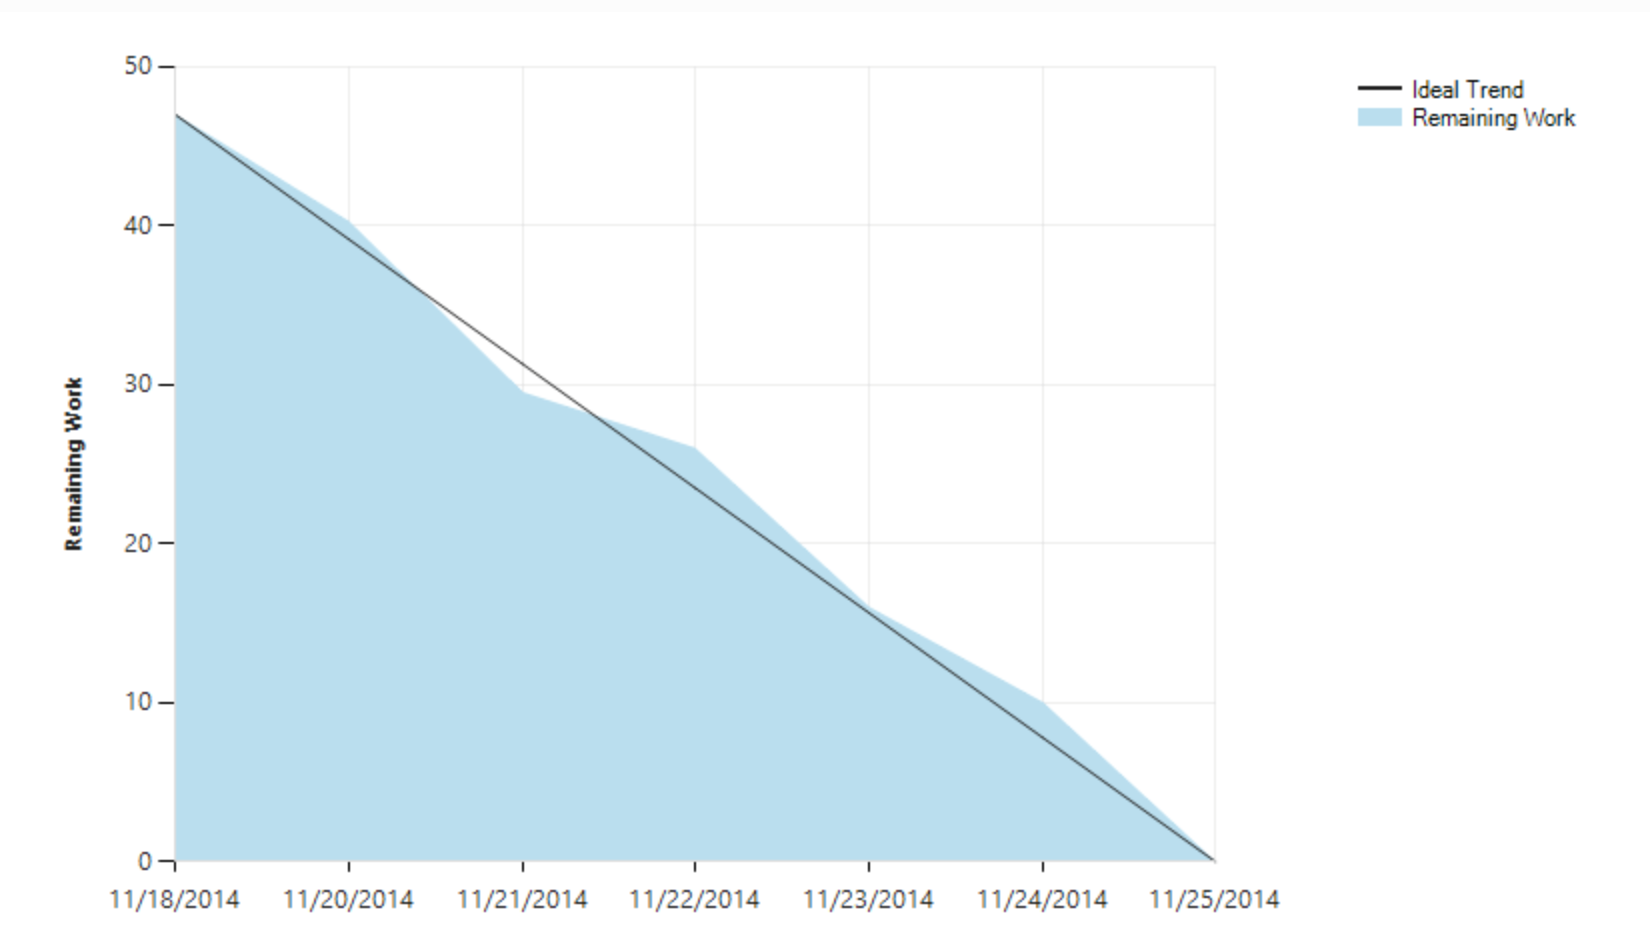
\includegraphics[scale=0.40]{Figures/Burndown1}
	% place the figure in the Figures folder (located with the main file)
	% you need to fix the scale a few times to get it right, but latex does not compress so one can always zoom in to see details.
	\caption{Burndown Chart of Sprint 1.}
\end{figure}

\subsection{Sprint 2}
The burndown chart after sprint two reflects how the team changed tactics. \\
It was decided at the sprint planning meeting after sprint one to have an aggressive amount of work assigned to every team member, in order to complete a larger amount of work. \\
Team members discussed not being able to complete \textit{every} task and focus on having a working prototype ready for the end of the sprint.\\
Note the total amount of hours at the top of the chart and the hump near the end. Also note that the team did not complete every assignment, but got the main tasks out of the way.

\begin{figure}[H]
	\centering
	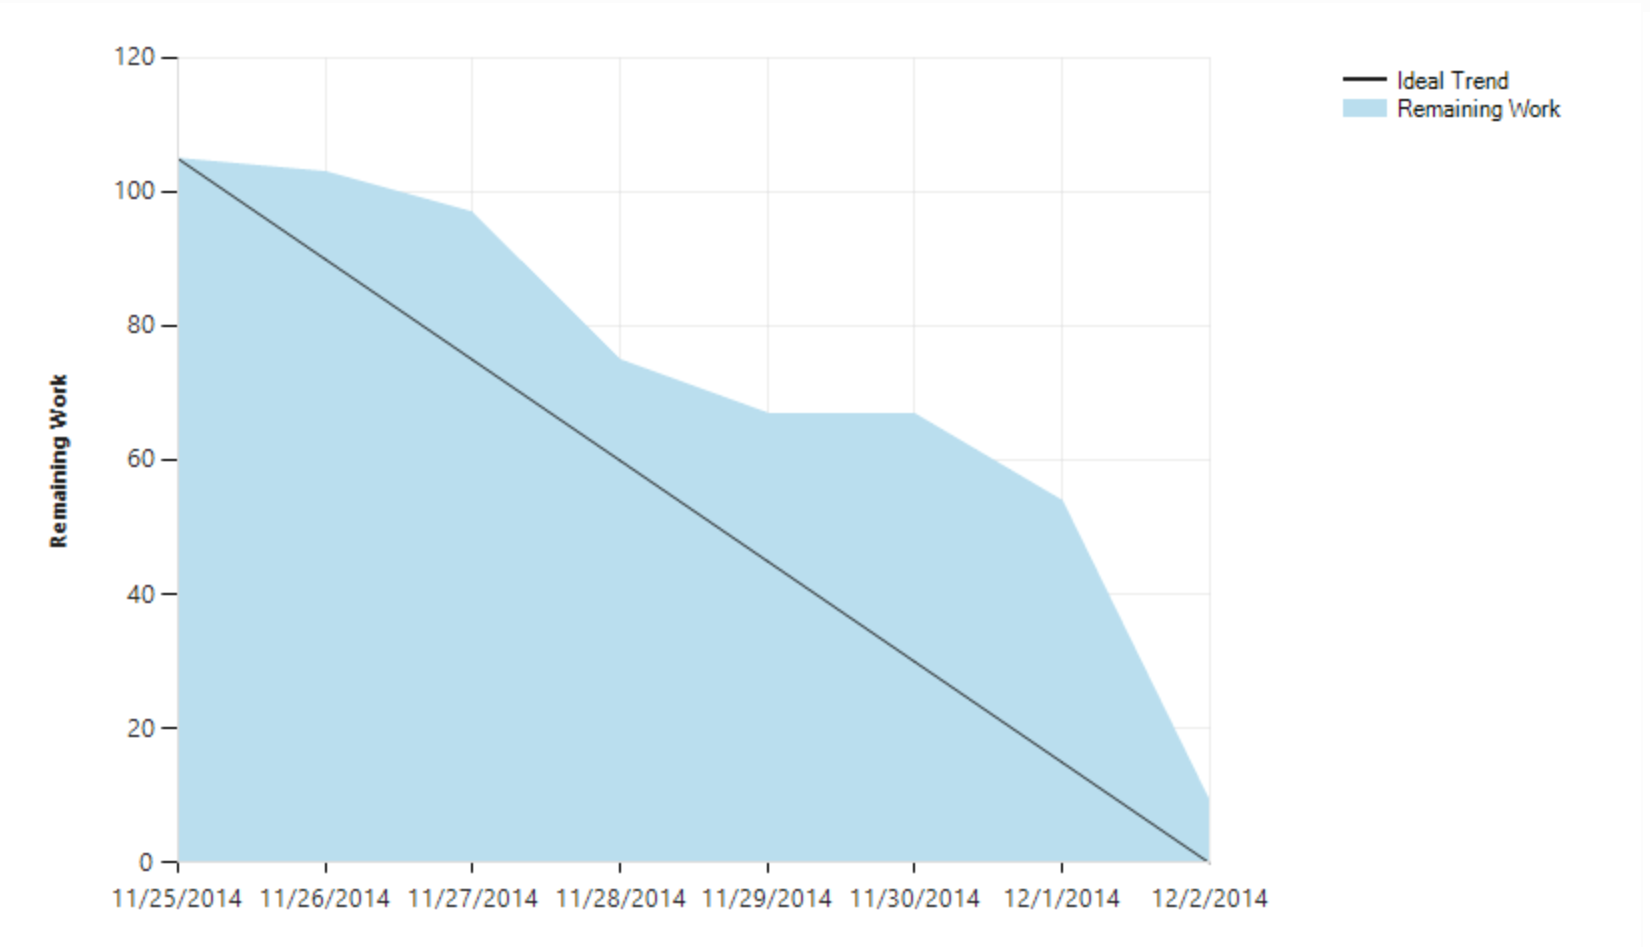
\includegraphics[scale=0.40]{Figures/Burndown2}
	% place the figure in the Figures folder (located with the main file)
	% you need to fix the scale a few times to get it right, but latex does not compress so one can always zoom in to see details.
	\caption{Burndown Chart of Sprint 2.}
\end{figure}

\subsection{Sprint 3}
The burndown chart after sprint three reflects how the team found a reasonable amount of work. \\
After having finished a working prototype the workload returned to a more "relaxed" amount.

\begin{figure}[H]
	\centering
	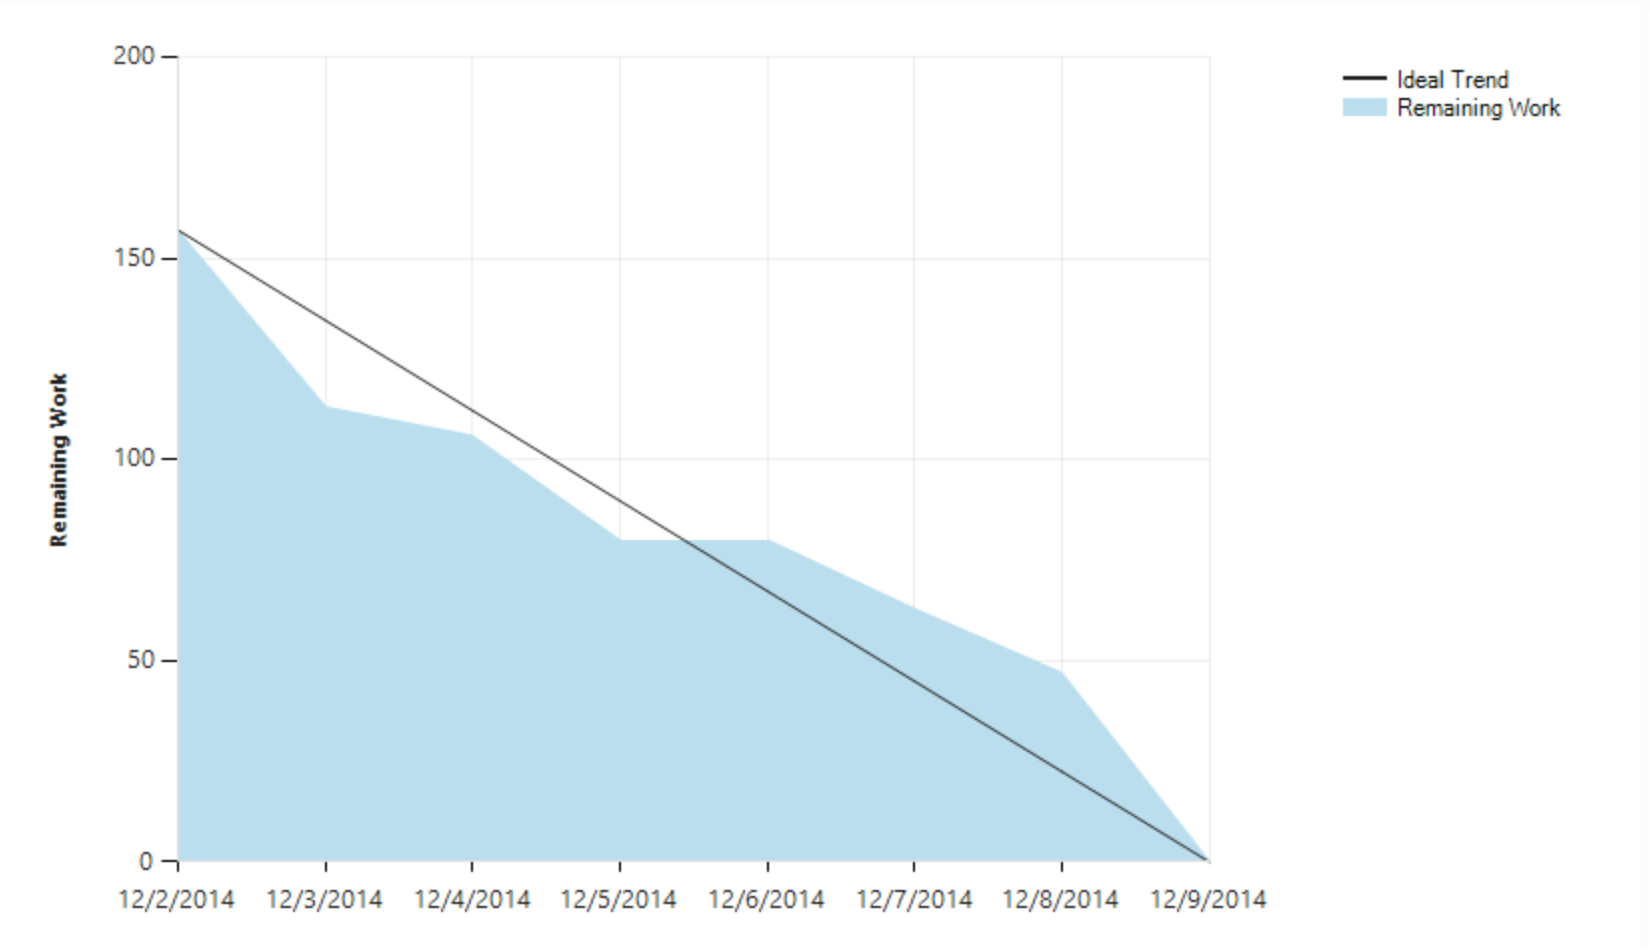
\includegraphics[scale=0.40]{Figures/Burndown3}
	% place the figure in the Figures folder (located with the main file)
	% you need to fix the scale a few times to get it right, but latex does not compress so one can always zoom in to see details.
	\caption{Burndown Chart of Sprint 3.}
\end{figure}

\subsection{Sprint 4}
The burndown chart after sprint four reflects how the team didn't use the online SCRUM tool and instead worked on items they felt needed work to be finished. The burndown chart reflects this in that it does not follow the expected graph. All work was finished, but sometimes not put into the system.\todo{change the figure} \\

\begin{figure}[H]
	\centering
	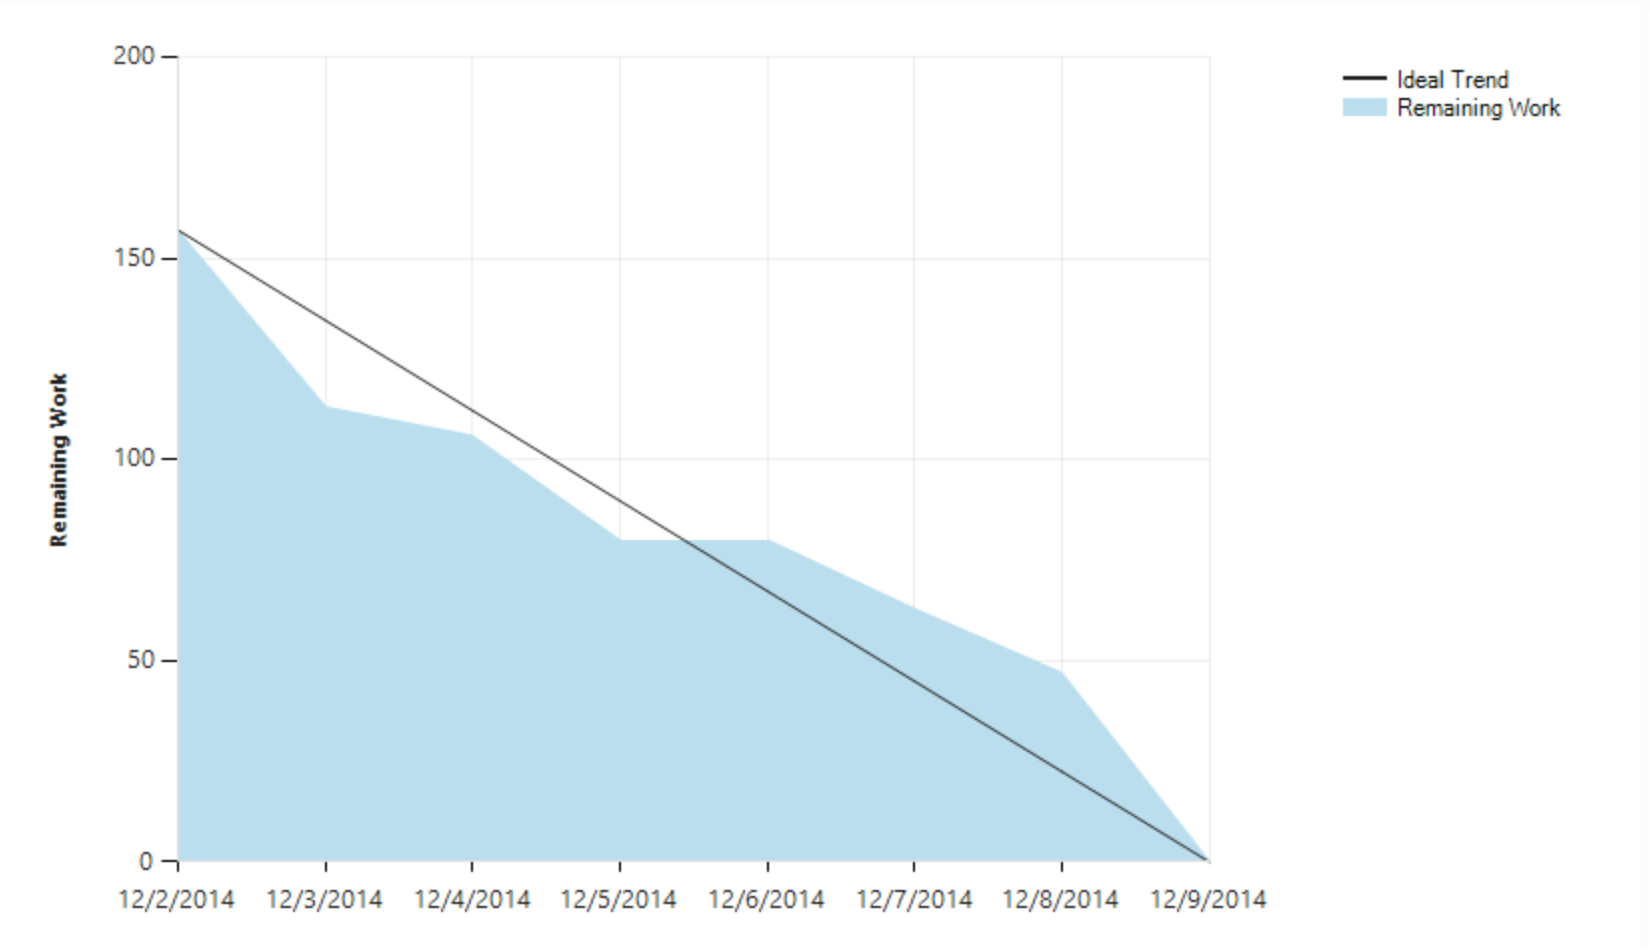
\includegraphics[scale=0.40]{Figures/Burndown3}
	% place the figure in the Figures folder (located with the main file)
	% you need to fix the scale a few times to get it right, but latex does not compress so one can always zoom in to see details.
	\caption{Burndown Chart of Sprint 4.}
\end{figure}
\section{Review and Retrospective}

Generally the retrospective meetings were finished very quickly.

The team worked quite well and did not face any major issues during the sprints.

The main issues found were the work estimates, where some tasks took longer or less time than expected and some team members allocated either too much or too little to themselves.

Focusing on the documentation in the first sprint gave the team a solid foundation for the ensuing programming sprints, which was a great benefit.

Using \textit{SCRUM} proved to be very effective in planning the work. Having shorter sprints helped keep spirits up for team members, and ensured that everyone did not drown in work. The team was always able to see the end of the next sprint and how much work was left.

Using an iterative approach was a benefit and the team appreciated the ability to change course during the project.

Having a waterfall-like approach would not have given the team the same abilities to do this, and unexpected problems that were discovered during the project might not have been as easy to fix.

The fact that the team was relatively small and therefore well-suited for the \textit{SCRUM} methodology helped a great deal as well. Had the team been larger other issues might have surfaced, which the waterfall approach would have handled better.

At the end of the project the team got a bit more relaxed assigning tasks before starting work. This resulted in some team members shifting focus, and working on tasks other than ones assigned to them. This resulted in a lack of overview, and some tasks getting pushed to end of the project.

This goes to show that sticking to the \textit{SCRUM} principles pays off, which the team forgot in the end, and even though \textit{SCRUM} seems as a more relaxed way of organising a team, you still need to follow the principles.\\

The project as an entirety has been a great success, and the \textit{SCRUM} methodology has proven a most valuable tool.
\part{Appendices List}
\chapter{Appendices}
\section{Appendix 1 - Distribution of Work}
\emph{Waiting for Bardram to upload his latex magic}
\section{Appendix for unspecified use case models}
\label{sec:unspecified_use_case_models}

List of use cases not specified further.
\begin{itemize}
    \item Contact interested customer
    \item Update car information
    \item Remove car from car lot database
    \item Search for cars that are up for sale
    \item Search for customers
    \item View orders
    \item Register a calling customer in the system
    \item Customer wants to delete account
    \item Customer wants to see cars with some specified specification
    \item A new employee is hired and must be added to the system
    \item An employee stops working at DriveIT and must be deleted from the system
    \item Information about an employee must be updated.
\end{itemize}

\section{Appendix for Sprint Retrospections}
\label{sec:scrum-sprints}
\subsubsection{Sprint 1: Retrospection}
\label{sec:sprint1}
\small{\textit{Facilitated by Jacob Stenum Czepluch (SCRUM master)}} 

\textbf{What Could Be Improved?}

\begin{itemize}
	\item Mikael would like to be able to see stuff in VS Online. He had no access.
	\item LaTeX is horrible, no one likes using it.
	\item TeX templates are weird and we spent time figuring them out.
	\item Markdown would make (at least Fischer's) life easier. 
	\item LaTeX conventions need to be specified and \textbf{used}. This takes time.
	\item Wind does not want to be the "tex-guy". Everyone needs to LaTeX their own stuff.
\end{itemize}

\textbf{What Went Well?}

\begin{itemize}
	\item Work went well. 
	\item People managed their time well.
	\item The workload will increase when coding starts.
	\item Facebook group worked really well.
	\item Tasks and SCRUM interface online works well.
	\item Graphical online interface gives a nice overview.
	\item Git works, branching is going to be interesting. 
\end{itemize}

\textbf{Presentation of Work}

We have no product owner, so the group therefore pretended to be the group owner while also being the developers of the product. 

All group members have checked the work together, and everything looks the way it should. \\
Minor improvements have either been made or planned and added to the next sprint. 


\subsubsection{Sprint 2: Retrospection}
\label{sec:sprint2}
\small{\textit{Facilitated by Anders Wind Steffensen (SCRUM master)}} 

\textbf{What Could Be Improved?}

\begin{itemize}
	\item Everyone would like a bit more time, but still felt they finished the most important work.
	\item Git branching is okay, some people still don't quite get it, but we have not had any major conflicts.
	\item We forgot the documentation a bit this time, focusing more on code. 
	\item Some group members underestimated the time they thought they would spend to finish a task.
	\item We need to remember to update the SCRUM online tool so that the burndown chart is correct.
	\item Visual Studio can be a bitch. There's too much black magic.
\end{itemize}

\textbf{What Went Well?}

\begin{itemize}
	\item Work went well. We managed to accomplish the major goals (working prototype).
	\item People managed their time well.
	\item Facebook group still works really well.
	\item Git is awesome when it works.
\end{itemize}

\textbf{Presentation of Work}

We have no product owner, so the group therefore pretended to be the group owner while also being the developer of the product.

All group members have checked the work together, and everything looks the way it should.\\
Minor improvements have either been made or planned and added to the next sprint, with mostly the same people assigned.\\
Work people didn't have time to finish have been added to the next sprint.

\subsubsection{Sprint 3: Retrospection}
\label{sec:sprint3}
\small{\textit{Facilitated by Anders Fischer-Nielsen (SCRUM master)}} 

\textbf{What Could Be Improved?}

\begin{itemize}
	\item We need to stay on top of updating the SCRUM tool (VS Online).
	\item We need a better delegation of work. Some group members relaxed a bit. 
	\subitem Better time estimates could fix this.
	\item The placement of big tasks (that affect other parts of the product) should be changed so that these happen at the beginning of the sprint. That should free up other team members so that they are less stressed by the end of a sprint. 
	\item We need to get better at attending the stand up meetings.  
	\item Noone should be working at the SCRUM meetings. \text{NO CODING!}
\end{itemize}

\textbf{What Went Well?}

\begin{itemize}
	\item The group is somewhat following the time frame for the product. We're not \textit{too} far behind so far.
	\item Time estimates are generally okay, everything considered. 
	\item The communication of the group is fine. The Facebook group is working beautifully. 
\end{itemize}

\textbf{Presentation of Work}

We have no product owner, so the group therefore pretended to be the group owner while also being the developer of the product.

Some group members have presented their finished work and eveything that people finished in time looks good.\\
Some tasks were not completed, and did not work, when we tried to show them off. 
Minor improvements have either been planned and added to the next sprint, with mostly the same people assigned.\\
The work group members didn't have time to finish have been added to the next sprint.\\

\subsubsection{Sprint 4: Retrospection}
\label{sec:sprint4}
\small{\textit{Facilitated by Anders Fischer-Nielsen (SCRUM master)}} 

\textbf{What Could Be Improved?}

\begin{itemize}
	\item Assigning tasks completely failed this sprint. Group members worked on whatever they felt was missing.
	\item We need a better delegation of work. Since members had no work assigned, roles were never assigned.
\end{itemize}

\textbf{What Went Well?}

\begin{itemize}
	\item Considering no tasks were delegated all the work was completed without major issues. 
	\item Work was finished in time in a satisfactory manner. Of course there were some things that could have been fixed post-project, but they are outside of the scope. 
\end{itemize}

\textbf{Presentation of Work}

We have no product owner, so the group therefore pretended to be the group owner while also being the developer of the product.

The team went through the finished work together, trying to find any missing requirements. 
No major issues were found. The work was deemed satisfactory (shippable) considering the time frame.

\section{Appendix for Github Repository}
All code is available on the private Github Repository: \url{https://github.com/andersfischernielsen/DriveIT}. Invitations to join the repository will be sent to Jakob Bardram and Rasmus Nielsen.



\end{document}